%%%%%%%%%%%%%%%%%%%%%%%%%%%
%                         %
%       2016.11.16.       %
%      Szakdolgozat       %
%    Tamás     LATEX      %
%%%%%%%%%%%%%%%%%%%%%%%%%%%
\documentclass[oneside,titlepage,12pt,a4paper]{report}
%\documentclass[12pt]{report}
\usepackage[centertags]{amsmath}
\usepackage{amsfonts}
\usepackage{amsthm}
\usepackage{newlfont}
%\usepackage[ansinew]{inputenc}
\usepackage[magyar]{babel}	
\usepackage[utf8]{inputenc}		
\usepackage{t1enc}				
\usepackage{graphicx}
\usepackage{color}
%\usepackage[colorlinks]{hyperref}
%\usepackage[active,new,noold,marker]{xrcs}
\usepackage{euler}
\usepackage{amssymb,latexsym}
\usepackage{amsmath}
\usepackage{graphics}
\usepackage{algorithm} 
%\usepackage{algpseudocode} %ezzel összeakadhat \usepackage{algorithmic} 
\usepackage{algorithmic} 
\usepackage{rotating}
\usepackage{bigstrut}
\usepackage{subfigure}
\usepackage{appendix}
\usepackage{setspace}


\newtheorem{theorem}{Theorem}
\newtheorem{corollary}{Corollary}
\newtheorem{lemma}{Lemma}
\newtheorem{proposition}{Proposition}
\newtheorem{definition}{Definition}
\newtheorem{notation}{Notation}

\textwidth=6.truein \textheight=9.truein \hoffset=-.5truein
\voffset=-.8truein

\frenchspacing				
\setlength{\parskip}{\smallskipamount}	
\renewcommand{\appendixtocname}{Függelék}
\renewcommand{\appendixpagename}{Függelék}
\DeclareMathOperator{\grad}{grad}
\DeclareMathOperator{\sgn}{sign}
\DeclareMathOperator{\PRD}{PRD}
\DeclareMathOperator{\CR}{CR}
\newcommand{\conj}[1]{\overline{#1}}

\begin{document}
\begin{titlepage}
	\parbox[t]{5.5cm}{\vspace{1cm}}
\begin{center}
	\large
	\textsc{Eötvös Loránd Tudományegyetem \linebreak Informatikai Kar} \\[2cm]
\end{center}

\begin{center}
	% Title
	\LARGE EKG jelek feldolgozása Hermite-függvények segítségével\\[0.55cm]
	\large BSc Szakdolgozat \\[1.9cm]
\end{center}

\begin{center}
	\parbox[t]{25mm}{Készítette:}
	\parbox[t]{5.5cm}
		{Dózsa Tamás\\
		ELTE IK\\
		Programtervező informatikus \\
		BSc
		}
	\\[0.9cm]
	
  \parbox[t]{25mm}{Témavezető:}
	\parbox[t]{5.5cm}{
		Dr. Kovács Péter\\
		Adjunktus\\
		ELTE IK\\
		Numerikus Analízis Tanszék
		}
	\\[4cm]
\end{center}

\begin{center}
	
\includegraphics[scale=0.7]{./Abrak/Egyeb/elte_logo.jpg}\\[1cm]
	Budapest, 2016.11.16.
\end{center}
\end{titlepage}

\tableofcontents

%%%%%%%%%%%%%%%%%%%%%
% BEVEZETES
%%%%%%%%%%%%%%%%%%%%%

\chapter{Bevezetés}
\label{intro}



\par
Az információ ábrázolásának módja az informatika tudomány fontos kérdése. Természetesen annak eldöntése, hogy egy adott adat halmaz milyen módon kerül ábrázolásra erősen függ annak jellegétől. Az adatábrázolás felel az adatok hatékony felhasználhatóságáért (például egy internetes video hívásnál az adatokat gyorsan kell egymás után továbbítani), ugyanakkor biztosítania kell, hogy az adatokból kinyerhető információ nem veszik el (ha túl rossz mindőségű képeket továbbítunk, a fogadó fél nem tudja értelmezni azokat). 
\par	A szakdolgozat célja egy speciális adatábrázolás, nevezetesen EKG jelek egy ábrázolásának bemutatása. Mivel jellemzően ezeket az adatokat, későbbiekben \textit{jelek}-et, általában nagyobb memória felhasználásával szokás ábrázolni, ezért a dolgozat az eljárásra EKG jelek \textit{tömörítéseként} hivatkozik. EKG jelek esetén az ábrázolás minősége sok szemponttól függ. Mivel ezek a jelek fontos információkat hordoznak a szív állapotáról, különösen fontos, hogy a tömörítés során ne vesszen el fontos információ. Egy ilyen jel rögzítésekor azonban sok olyan adat is tárolásra kerül (például a végtagok mérés közbeni mozgatása miatt), amelyek nem hordoznak fontos információt. Az ilyen adatokra a dolgozat \textit{zaj}-ként hivatkozik. Egy jó EKG ábrázolás sikeresen szűri a mérés során keletkezett zajt, miközben az orvosi szempontból fontosnak nevezhető információt megtartja. Mivel a dolgozatban egy tömörítési eljárás kerül bemutatásra, fontos szempont az EKG jelek memória takarékos ábrázolása. Gyakorlati szempontból minél kevesebb memórián történik meg a jelek ábrázolása, annál könnyebb azokat tárolni (hosszú mérések esetén fontos lehet), illetve egyszerűbb és biztonságosabb a jelek hálózaton törtenő továbbítása. EKG jeleknek egy igazán jónak nevezhető ábrázolása pedig az eddig említettek mellett az orvosok munkáját közvetlenül segítő információt is kódol magában. Ilyen lehet például egy olyan ábrázolás amely hatékony bemenetéül szolgál valamilyen osztályozó algoritmusnak, lehetővé téve az abnormális jelek automatikus felismerését. 
	\par A dolgozat három fő fejezetre tagolható. A Bevezetés című fejezetben található a dolgozatban bemutatott eljárás specifikációja, a jel reprezentáció matematikai modelljének ismertetése, valamint a bemutatott módszer egyéb jellemzőit ismertető alfejezetek. Ezek közé tartozik például a jel közelítésének optimalizációjához szükséges Nelder-Mead algoritmus elméleti bemutatása, illetve az EKG jel szegmentációját elősegítő Matching-Pursuit algoritmust részletező alfejezet. 
\par	A dolgozat második fejezete az eljárás mellékelt implementációjának a fejlesztői dokumentációja. Ebben a fejezetben találhatóak a tömörítő eljárást implementáló c++ osztályok jellemzői, illetve az elérést segítő webes felület implementációjának részletes ismertetése. A fejlesztői dokumentáció fejezet tartalmazza továbbá a program logikai jellemzését elősegítő UML és egyéb osztálydiagrammokat. A fejezet igyekszik pragmatikusan és érthetően jellemezni a program felépítését, illetve kellően megindokolni az egyes implementációk mellett szóló döntéseket. 
\par	A Felhasználói dokumentáció fejezetbe, a program használatával kapcsolatos információk kerültek. Ebben a fejezetben található a felhasználói felület funkcióinak pontos ismertetése, valamint hasznos példák annak használatára. Bemutatásra kerülnek továbbá a program használatához szükséges előkészületi lépések, és az ismert rendszerkövetelmények. 
\par	A dolgozat utolsó része a függelék, melyben a Bevezetés fejezetben található matematikai állítások bizonyításai, egyéb kapcsolódó matematikai fogalmak leírásai, illetve felhasznált algoritmusok pszeudo-kódja található. 
		
\section{A feladat specifikációja}

A dolgozat célja egy olyan tömörítési eljárás bemutatása, amely lehetővé teszi az EKG jelek hatékony (memória takarékos) ábrázolását, a mérések zaj szűrését, illetve az EKG hullámszegmenseinek szeparációját. Az utóbbi jellemző orvosi szempontból lehet hasznos, ugyanis sok kóros elváltozás kimutatásához szükséges az egyes hullámszegmensek széleinek ismerete. A dolgozatban bemutatott módszer hatékonysága, az irodalomban fellelhető más tömörítési eljárások \cite{} hatékonyságának összehasonlításával igazolandó. \par A dolgozatban bemutatott tömörítési eljárás implementációjának feladata, hogy az MIT-BIH adatbázisban található EKG jelek tömörítésére alkalmas legyen, ehhez pedig egy könnyen használható webes felületet biztosítson. Az implementációnak két féle bemente megengedett: tömörítés esetén az MIT-BIH adatbázisban megtalálható EKG jelek, illetve a tömörítés következtében létrejött számsorozat, melyet a tömörített jel helyreállításához használ.  

\section{A modell ismertetése}
A modern orvostudományban nagy jelentőséggel bírnak 
a valamely élő szervezet által kibocsátott úgynevezett $biológiai jelek$. Ezek közé sorolható az $Elektro$ $Kardio$ $Gram$, vagy $EKG$,
amely a szív állapotáról képes információt adni. Bár ennek a dolgozatnak nem célja az $EKG$ jelek pontos elemzése, fontos néhány sorban ismertetni egy átlagos $EKG$ jel meghatározó hullámait. Egyetlen szí vütés  $EKG$ reprezentációja három fő részre bontható: a szí vütés elején megjelenő $P$ hullámra, az ezt követő $QRS$ komplexumra, és az ütés végén található $T$ hullámra. Ezek rendre a pitvari összehűzódást, a kamrák depolarizációját és elektromos újratöltődését reprezentálják. Diagnosztikai szempontból a $QRS$ komplexus a legfontosabb, ezért ezt nagy pontossággal kell tárolni. Általánosságban elmondható, hogy ezeknek a hullámoknak kezdő és végpontjai, valamint maximum és minimum értékei vesznek részt az orvosi diagnosztikában. Az említett paraméterek az \ref{fig:ekg} ábrán láthatóak.

\begin{figure}[htb!]
\begin{center}
   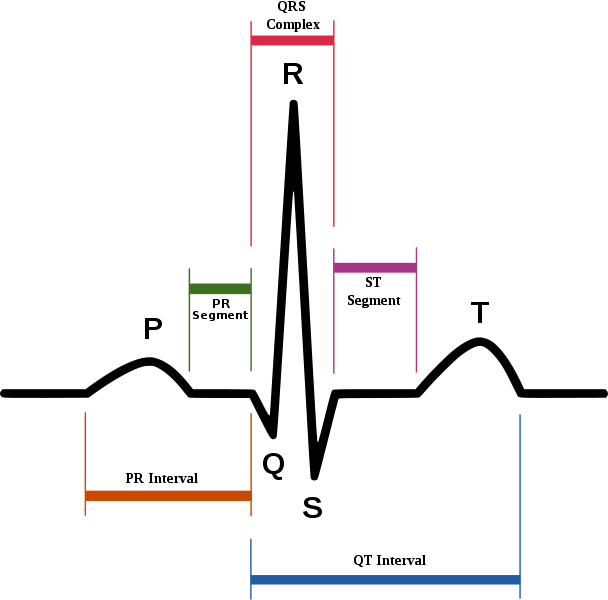
\includegraphics[scale=0.37]{./Abrak/Egyeb/ecg_wiki.png}
   \caption{Az EKG jel egy szívütése, illetve annak főbb diagnosztikai jellemzői.}
		\label{fig:ekg}
\end{center}
\end{figure}
 
Az irodalomban ismert tömörítő algoritmusokat \cite{unifiedReview} alapján három kategóriába sorolhatjuk: 1) egyszerű paraméteres becslések (pl.: interpoláció, különbségi kódolás, stb.), 2) direkt módszerek (pl.: csúcsok, meredekségek, stb. tárolása), 3) transzformációs eljárások. Az utóbbi osztály tartalmazza azokat az algoritmusokat, melyek a jelet egy előre adott függvényrendszer szerinti sorfejtéssel approximálják. Így az eredeti adatsorozat helyett csak az együtthatókat és a rendszer paramétereit kell tárolnunk. Ezen kategóriába sorolandó a dolgozatban bemutatott algoritmus is. Nevezetesen, az eredeti adatsorozatot speciális, Hermite-polinomok segítségével előállitott függvényrendszerrel fogjuk közelíti. A módszer alapját képező eljárás \cite{hexp3}, jól ismert az irodalomban, mely nem csak a jelek tömörítéséhez, de azok modellezéséhez \cite{hexp2}, illetve osztályozásához \cite{hexp1, hexp4} is alkalmazható. A dolgozatban az EKG jelekkel való hasonlóságuk miatt Hermite-függvényeket használunk az adatok reprezentálásához. Ezeket egy argumentum transzformáción keresztül szabad paraméterekkel egészítjük ki. Ennek köszönhetően az eredeti jelet egy adaptív bázisban írhatjuk fel. Az említett paraméterek megválasztásához a Nelder-Mead optimalizációs eljárást alkalmaztuk. Mivel az EKG jelek diszkrét adatsorozatok, ezért a módszert \cite{hexp5} alapján implementáltuk diszkrét ortogonális Hermite-polinomokra is. A dolgozatban különböző tesztekkel demonstráljuk az algoritmus hatékonyságát. Ehhez, több órányi, zajjal terhelt, valódi EKG felvételt használtunk. Ezen keresztül a bemutatott módszert összehasonlítottuk több másik, az irodalomban jól ismert tömörítő algoritmussal is \cite{jpeg2000ECG}. 

A tömörítő eljárást egy c++ nyelven megírt, objektum elvű alkalmazás implementálja, melyet egy webes felületen keresztül érhetünk el. A felület lehetőséget biztosít a dolgozatban jelölt tesztek újrafuttatására, valamint a teszteléskor felhasznált adatbázis további jeleinek a tömörítésére. Szintén a webes felületen keresztül nyílik alkamunk a már tömörített EKG jelek helyreállítására. 

Az alkalmazás megetrvezésekor külön hangsúlyt kapott a kód újra felhasználhatósága. Ennek érdekében a felhasznált algoritmusok, illetve matematikai modellek a lehető legáltalánosabb formában lettek implementálva. Fontos szempontot jelentett továbbá a c++11-es nyelvszabvány által nyújtotta lehetőségek minél hatékonyabb kihasználása. Jó példa erre a lambda függvények alkalmazása az optimalizációs algoritmusok implementációja során. A hatékony működés mellett azonban a program igyekszik megfelelni a modern felhasználók igényeinek. Ennek érdekében a felhaszálói felület weboldalként lett implementálva. A rendszerfüggetlen, és installáció mentes elérés lehetővé teszi a gyors és egyszerű használatot, valamint az eredmények megosztását.  

\section{Matematikai háttér}
\subsection{Jelek approximációja}

EKG jelek feldolgozásakor sok esetben szembesülünk gyakorlati kihívásokkal. Két sűrűn előforduló példa a hosszú mérések tárolása, valamint a zajjal terhelt mérések ábrázolása. Ezekre a nehézségekre egyszerre ad kielégítő megoldást, ha a jeleket  valamely $\mathcal H$ Hilbert-tér sima függvényeiből álló $(\Phi_n, n\in\Bbb N)$ ortogonális bázisában reprezentáljuk és a jelet véges sok $\Phi_0,\Phi_1,\cdots,\Phi_n$ bázisbeli elem lineáris kombinációjával közelítjük. Az $f\in\mathcal H$ jel
legjobb közelítését a tér $\|\cdot\|$ normájában az
$$
S_nf:=\sum_{k=0}^n\langle f,\Phi_k\rangle \Phi_k
$$
leképezés nyújtja, ahol $\langle\cdot,\cdot\rangle$ az $\mathcal  H$ tér
skaláris szorzatát jelöli. A jel és a közelítés eltérésének négyzete  a
$$
\|f-S_nf\|^2=\|f\|^2-\sum_{k=0}^n|\langle f,\Phi_k\rangle|^2
$$
képplettel adható meg. Adott hibán belüli közelítést véve a jel helyett  elég az
$S_nf$ approximációt reprezentáló  $\langle f,\Phi_k\rangle\ (k=0,1,\cdots, n)$ Fourier-együtthatókat tárolni.  Zajos jel esetén az ilyen típusú approximáció szűrőként is szolgál.  A közelítés megvalósításához a klasszikus ortogonális rendszerek közül  EKG görbék közelítésére  az Hermite-féle függvények bizonyultak használhatónak. Ezt támasztják alá a [...] dolgozatok. Az  Hermite függvények alkalmazása azzal is indikolható, hogy grafikonjuk hasonlít az EKG görbékre. Ezt a tulajdonságot a \ref{fig:phi0-3} ábra szemlélteti.

\iffalse

\begin{figure}
\centering
\subfigure[$\Phi_{0}(x)$]{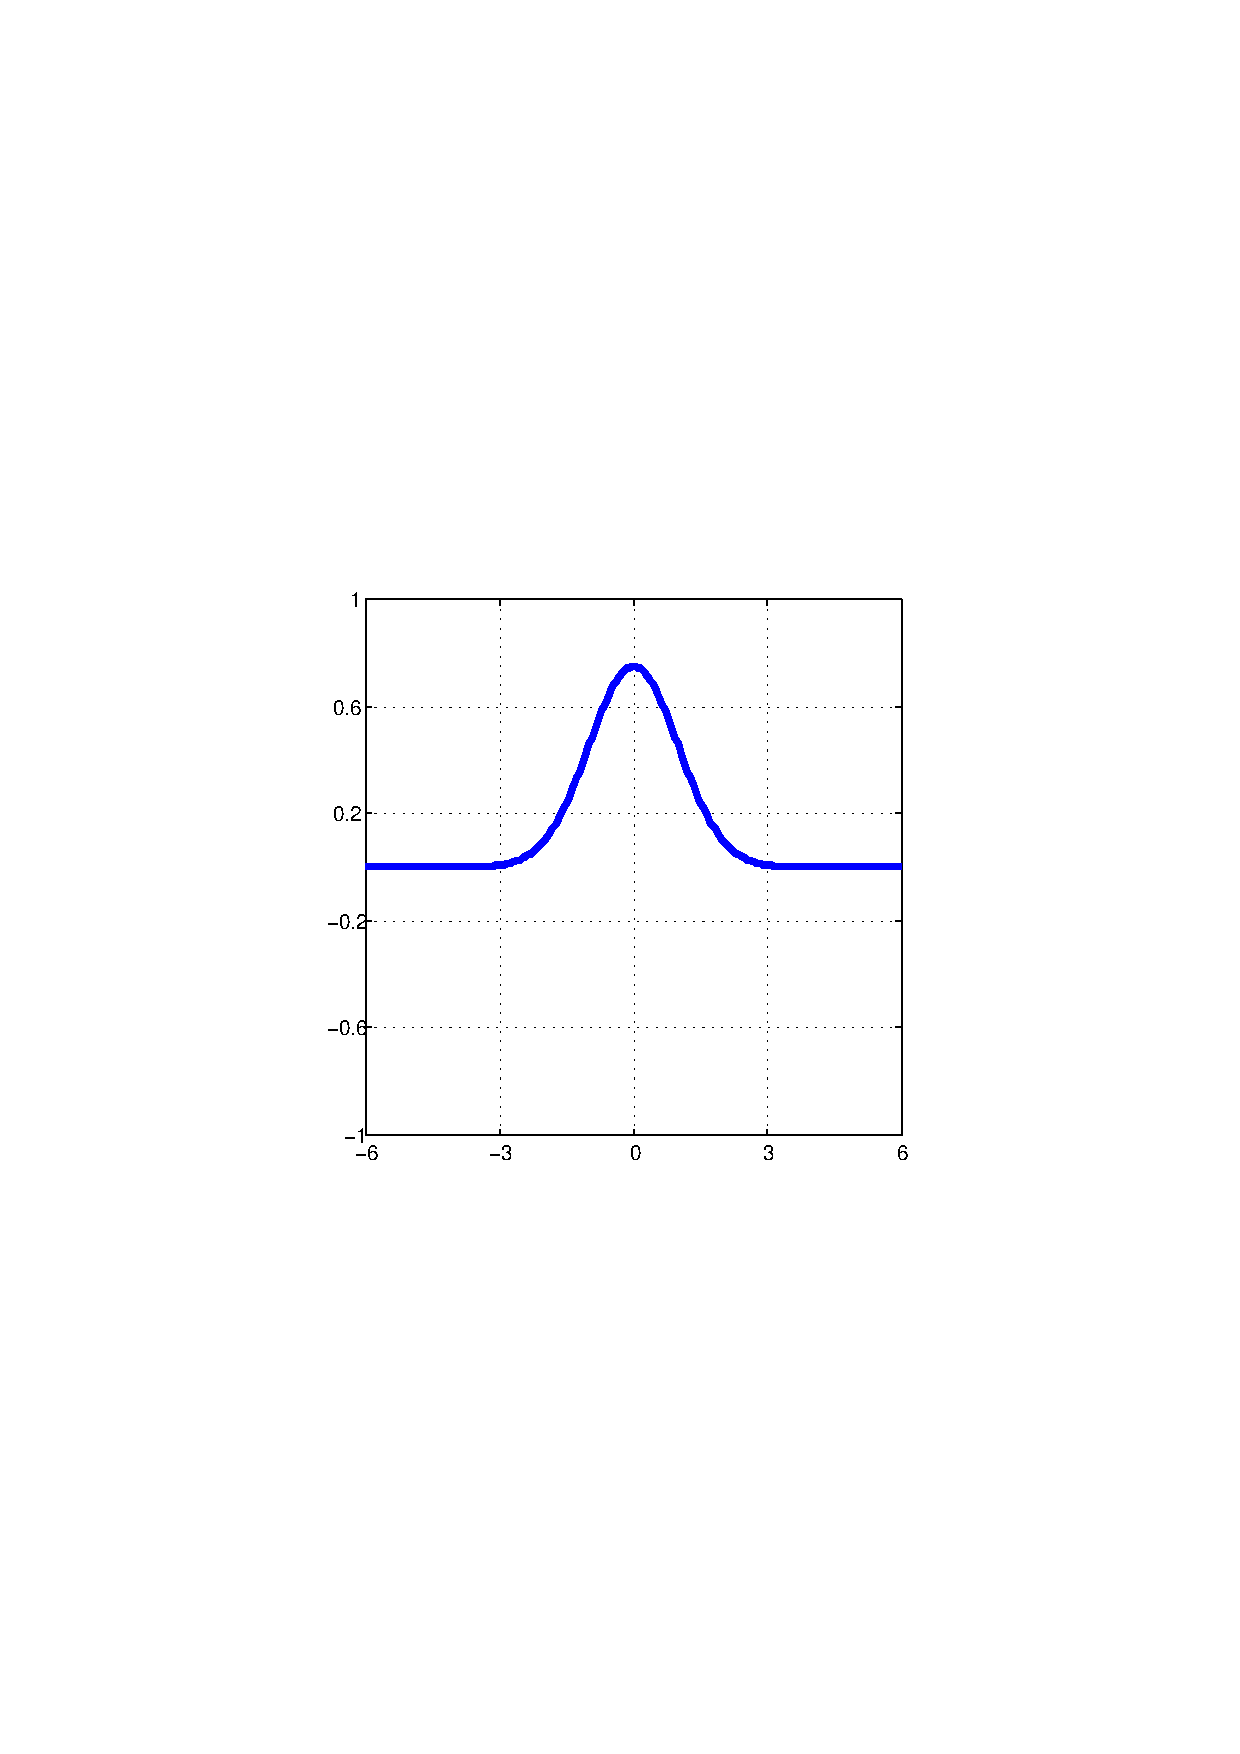
\includegraphics[scale=0.34,trim=150 280 150 280,clip]{./%Abrak/Egyeb/phi0.pdf}} 
\subfigure[$\Phi_{1}(x)$]{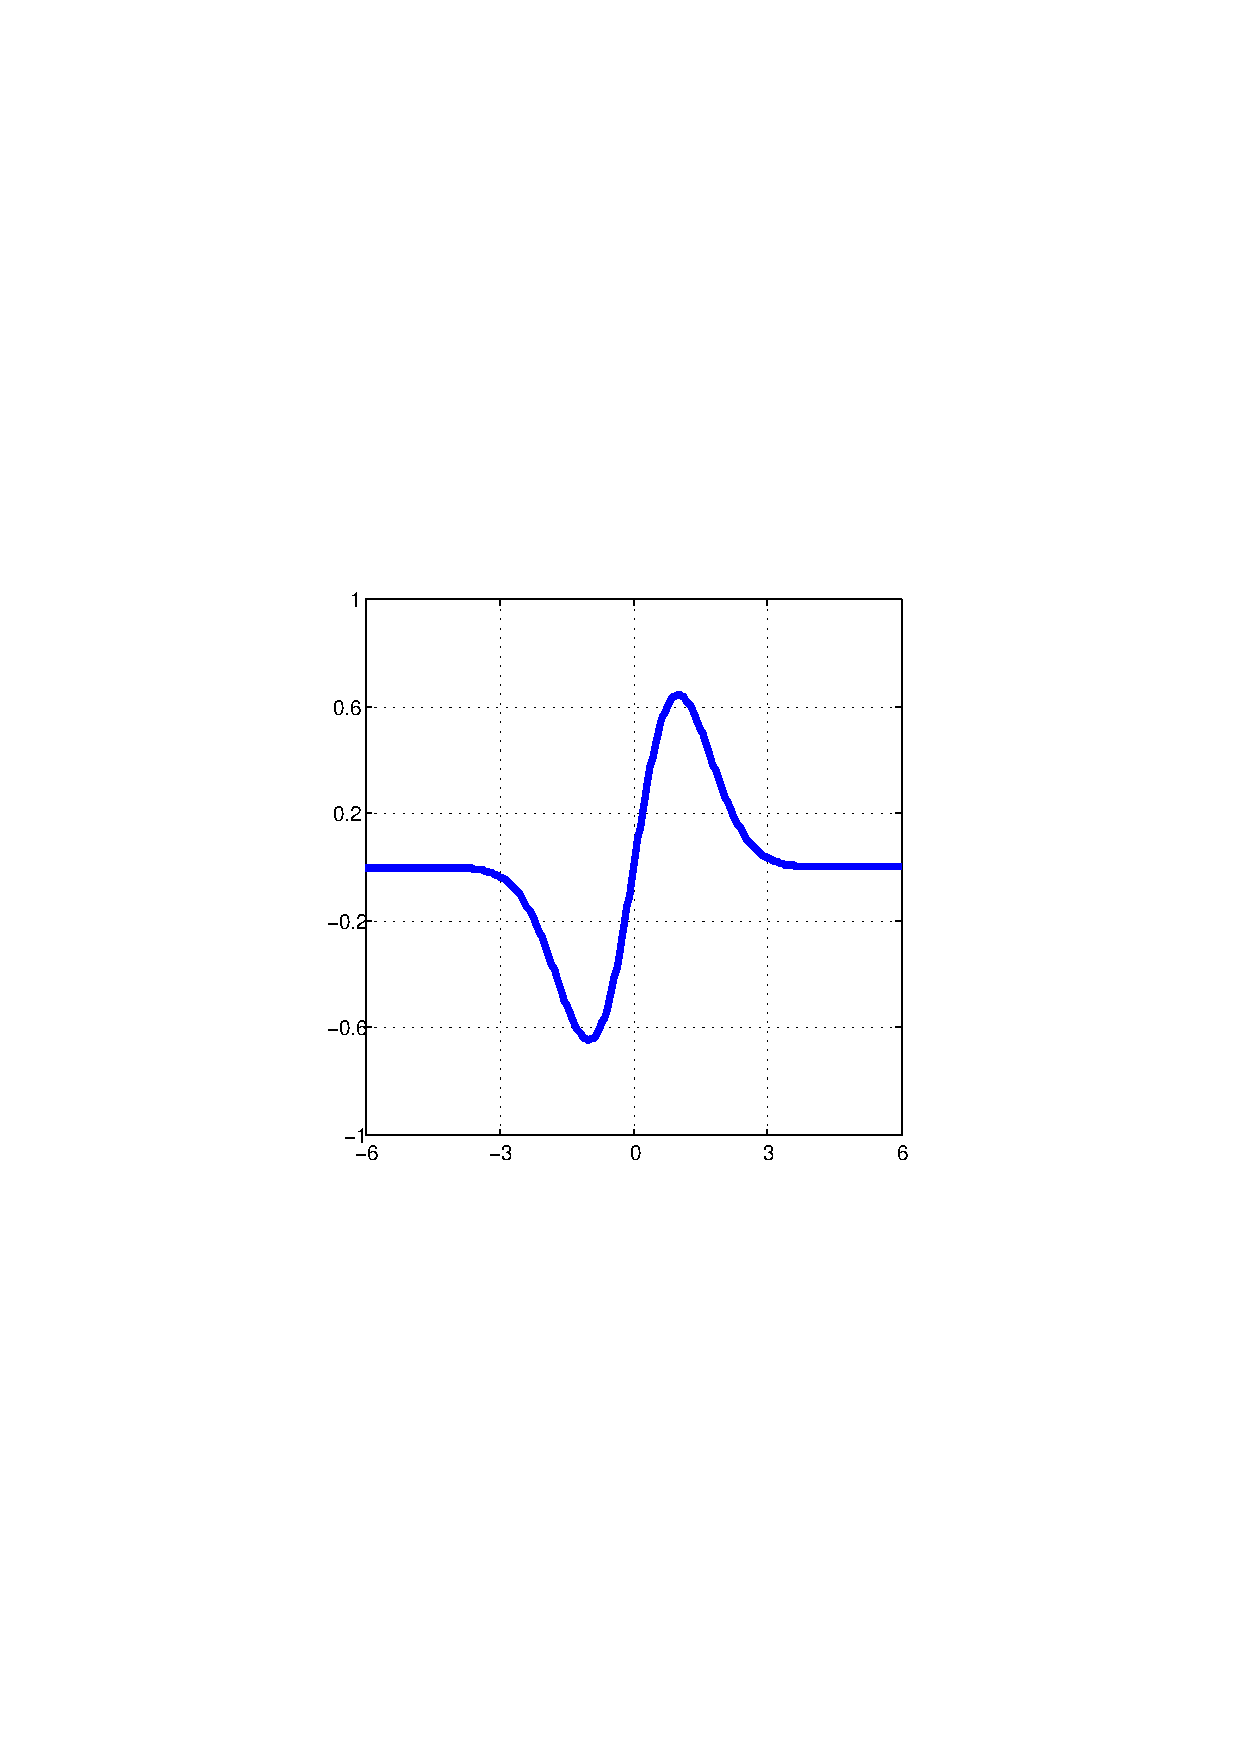
\includegraphics[scale=0.34,trim=150 280 150 280,clip]{./%Abrak/Egyeb/phi1.pdf}}
\subfigure[$\Phi_{2}(x)$]{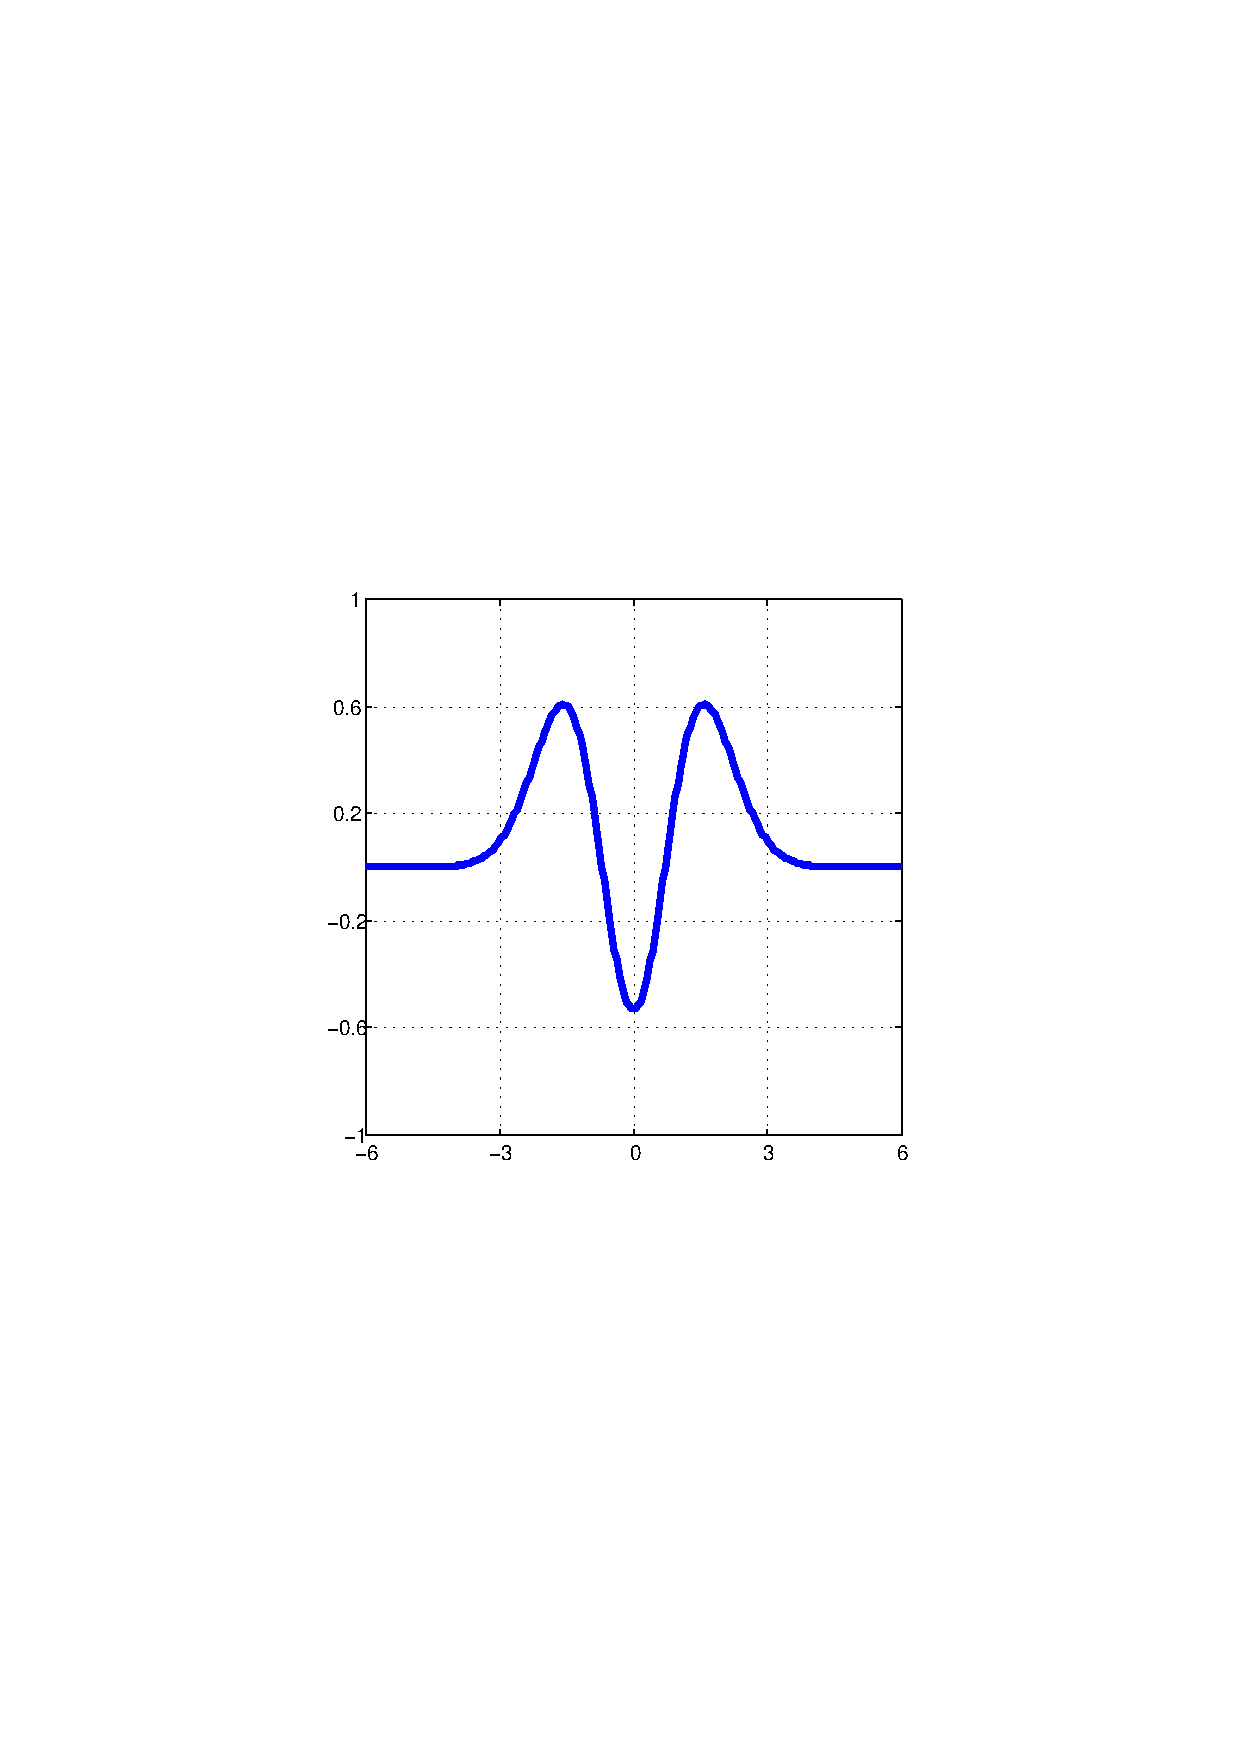
\includegraphics[scale=0.34,trim=150 280 150 280,clip]{./%Abrak/Egyeb/phi2.pdf}} 
\subfigure[$\Phi_{3}(x)$]{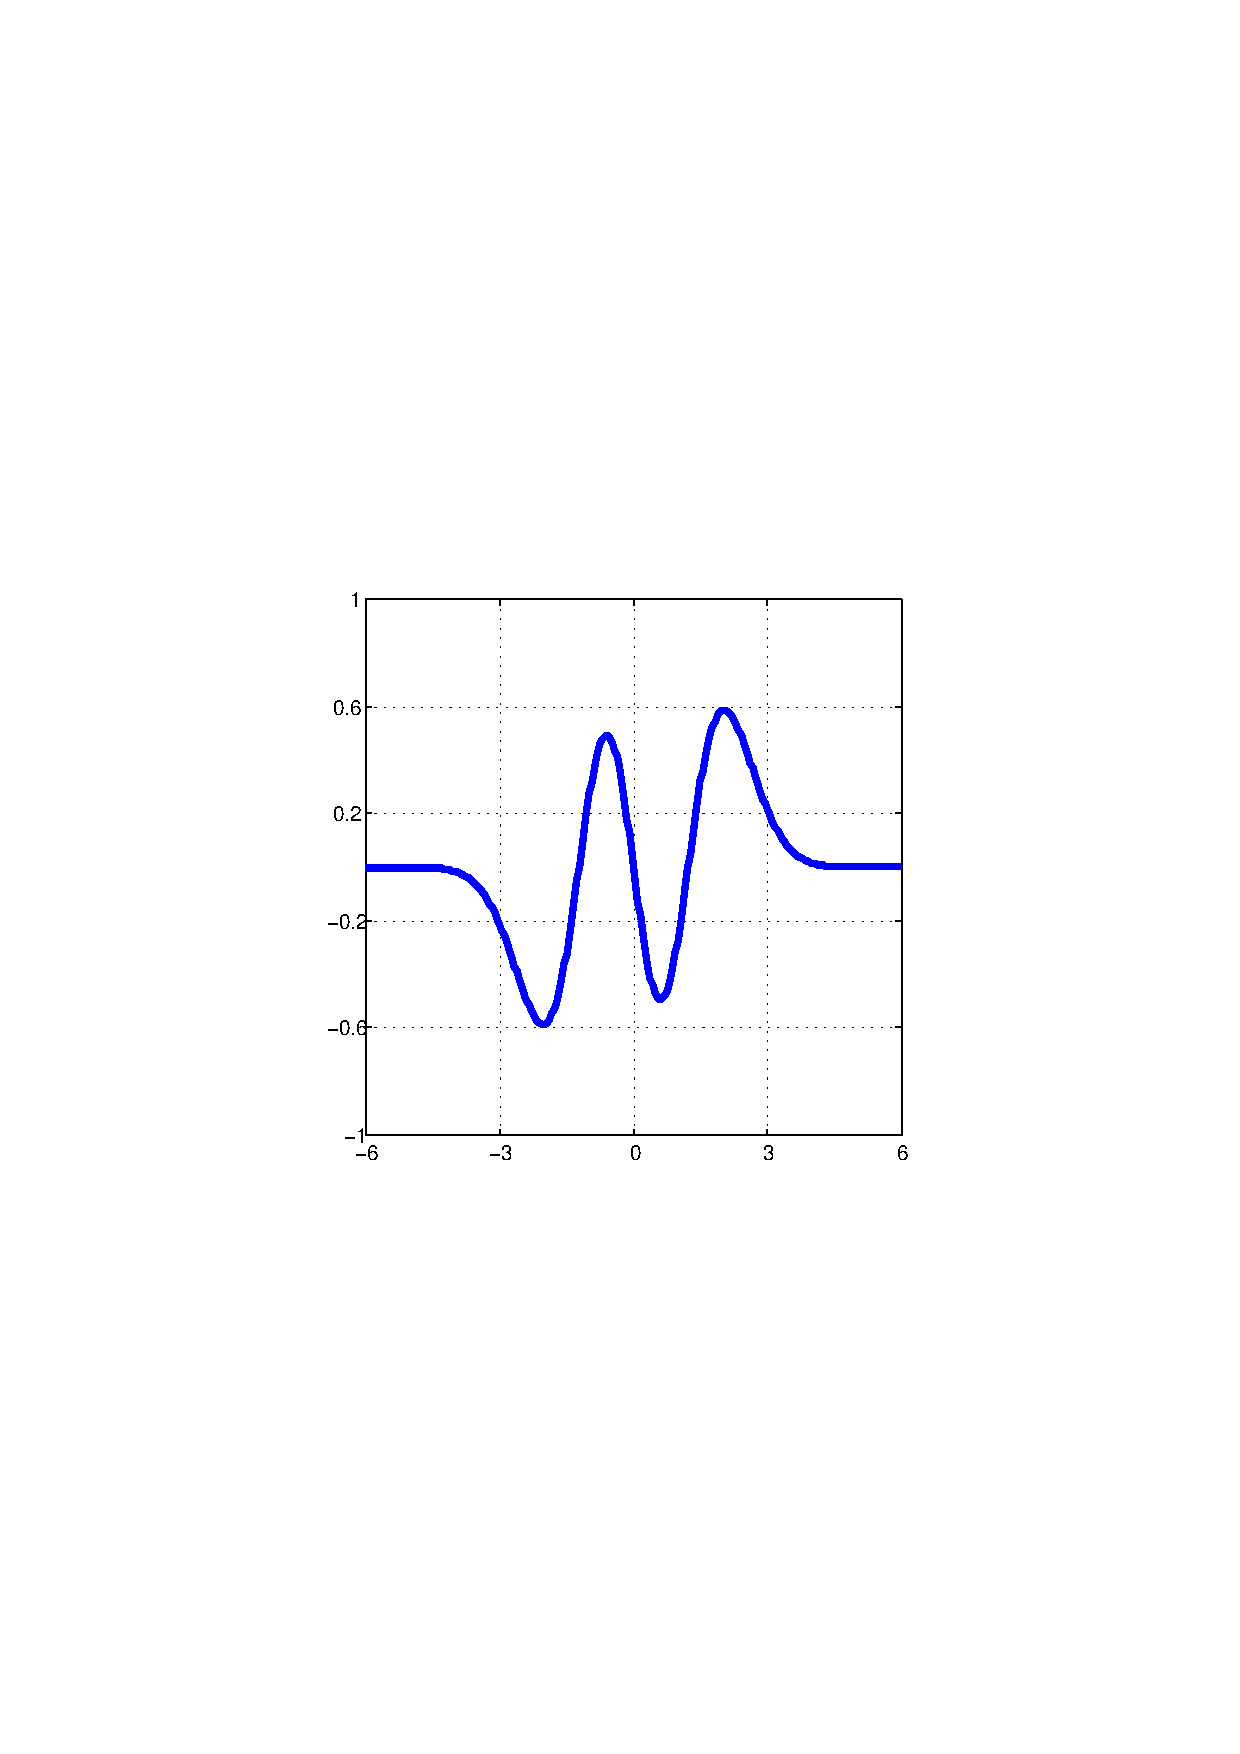
\includegraphics[scale=0.34,trim=150 280 150 280,clip]{./%Abrak/Egyeb/phi3.pdf}}
\caption{A Hermite-függvényrendszer első négy tagja.}
\label{fig:phi0-3}
\end{figure}
\fi


\subsection{Hermite-függvények}
A dolgozatban  az $\Bbb R$ számegyenesen (Lebesgue-mérték szerint) négyzetesen integrálható függvények $\mathcal H$ Hilbert-tere helyett elegendő a szakaszonként folytonos, az $\Bbb R$-en  négyzetesen integrálható függvények $\mathcal F$ euklideszi terét használni. Ebben a térben a skaláris szorzat és a norma a következő alakban írható fel:
\begin{equation}
 \langle f,g\rangle:=\int_{-\infty}^\infty f(t)g(t)\, dt,\ \ \|f\|:=\sqrt{\langle f,f\rangle}\ \ (f,g\in\mathcal F)\,.
\label{eq:dotprod}
\end{equation}
Továbbá, a
 \begin{equation*}
 \Phi_n(x):=H_n(x)e^{-x^2/2}/\sqrt{\pi^{1/2}2^n n!}\quad \ (n\in\Bbb N)
 \end{equation*}
normált Hermite-függvények (teljes) ortonormált rendszert alkotnak az $\mathcal F$ téren:
  \begin{equation*}
   \langle \Phi_n,\Phi_m\rangle=\delta_{nm}\ \ (m,n\in\Bbb N),\quad
  \|f-S_nf\|\to 0\ (n\to\infty)\,.
   \end{equation*}
Itt $H_n\ (n\in\Bbb N)$ jelöli az Hermite-féle polinomokat.
\\
\\
Az Hermite-függvények alkalmazásának számos előnye van: \\
\\
i) A $\Phi_n\ (n\in\Bbb N)$ rendszer zárt (teljes) az $\mathcal F$ téren. \\
\\
ii) A $\Phi_n(x)$ függvények gyorsan tartanak $0$-hoz, ha $|x|\to \infty$: \\
$$
|\Phi_n(x)|\le M_n e^{-x^2/4}\le M_n\ \ (x\in\Bbb R, n\in\Bbb N).
$$
\\
iii) A $\Phi_n$ függvények (stabil) másodrendű rekurzióval számíthatók: \\
\begin{equation}
\begin{split}
&\Phi_0(x):=e^{-x^2/2}/\pi^{1/4},\ \Phi_1(x):=\sqrt{2}\, x e^{-x^2/2}/\pi^{1/4}\\
&\Phi_n(x)=\sqrt{\frac 2 n} x \Phi_{n-1}(x)-\sqrt{\frac{n-1}n}\Phi_{n-2}(x)\ \ (x\in\Bbb R, n\ge 2)
\end{split}
\end{equation} 
\\
\\
iv) A $\Phi_n'$ deriváltak kifejezhetők a $\Phi_n, \Phi_{n-1} $ függvényekkel: \\
\begin{equation}
\Phi_n'(x)=\sqrt{2n}\Phi_{n-1}(x)-x\Phi_n(x)\ \ (x\in\Bbb R, n\in\Bbb N,\Phi_{-1}=0)
\end{equation}

\subsection{Az approximáció optimalizálása}

A jelek reprezentációja  függ az időskála $0$ pontjának és az egység
megválasztásától. Ezeket a paramétereket  a gyakorlatban önkényesen szoktuk
 megválasztani. Ezzel összefüggében felvethető a kérdés, hogyan lehet optimálisan megválaszthatani  ezeket a paramétereket.
Az  approximáció pontossága javítható azonos együttható szám mellett, amennyiben az  Hermite-függvények helyett azok
\begin{equation}
\Phi_n^{a,\lambda}(x):=\Phi_n(\lambda x+a)\ \  (x,a\in\Bbb R, \lambda>0)
\end{equation}
affin transzformáltjait használjuk. A $\sqrt{\lambda}\Phi_n^{a,\lambda}\ (n\in\Bbb N)$ rendszer is ortonormált és teljes az $\mathcal F$ téren. Ebben az esetben
az $f$ legjobb approximációja az
\begin{equation}
S_n^{a,\lambda}f:=\sum_{k=0}^n\langle f,\Phi_k^{a,\lambda}\rangle\Phi_k^{a,\lambda}\ \
(n\in\Bbb N, a\in\Bbb R,\lambda>0)
\end{equation}
projekció és a közelítés hibája az $a$ transzlációs és a $\lambda$ dilatációs paraméter függvénye:
\begin{equation}
D^2_n(a,\lambda):=\|f\|^2-\sum_{k=0}^n|\langle f,\Phi_k^{a,\lambda}\rangle|^2.
\end{equation}
            E két szabad paraméter optimalizálásával azonos együtthatószám mellett, az eredeti Hermite polinomokkal törtánő  approximációhoz képest pontosabb közelítés érhető el. A $D_n$ függvény minimalizálása ekvivalens  az
 $$
 F_n(a,\lambda):=\sum_{k=0}^n|\langle f,\Phi_k^{a,\lambda}\rangle|^2
 $$
 függvény maximumának meghatározásával. A paraméteres integrálok tulajdonságaiból következik, hogy az
 $$
 A_n(a,\lambda):=\langle f,\Phi_k^{a,\lambda}\rangle \ \  ((a,\lambda)\in T:=\Bbb R\times (0,\infty))
 $$
 Fourier-együtthatók a $T$ tartományon a paraméterek sima függvényei. Bebizonyítható, hogy $\lambda\to 0$ és $|a|+\lambda\to \infty$ esetén
 $F_k(a,\lambda)\to 0$, következésképpen az $F_n$ függvénynek létezik a
 maximuma és a $D_n$ függvénynek létezik a minimuma. A részleteket a Függelékben találhatók.

 Az alábbi ábrák az $F_n(a,\lambda)$ függvényeket szemléltetik fényintenzitás és perspektivikus ábrázolást használva. A harmadik ablakon
a jel közelí tését szemlélteti a maximum helynek megfelelő, ill.  egyéb
paraméter esetén.

\begin{figure}[H]
\begin{center}
   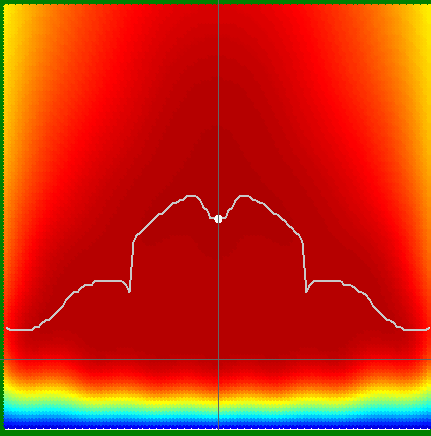
\includegraphics[width=100mm]{./Abrak/Ereszkedo1/F_2sz.png}
  \caption{Az $F_n$ szí nkódos ábrázolása}
\end{center}
\end{figure}

\begin{figure}[H]
\begin{center}
   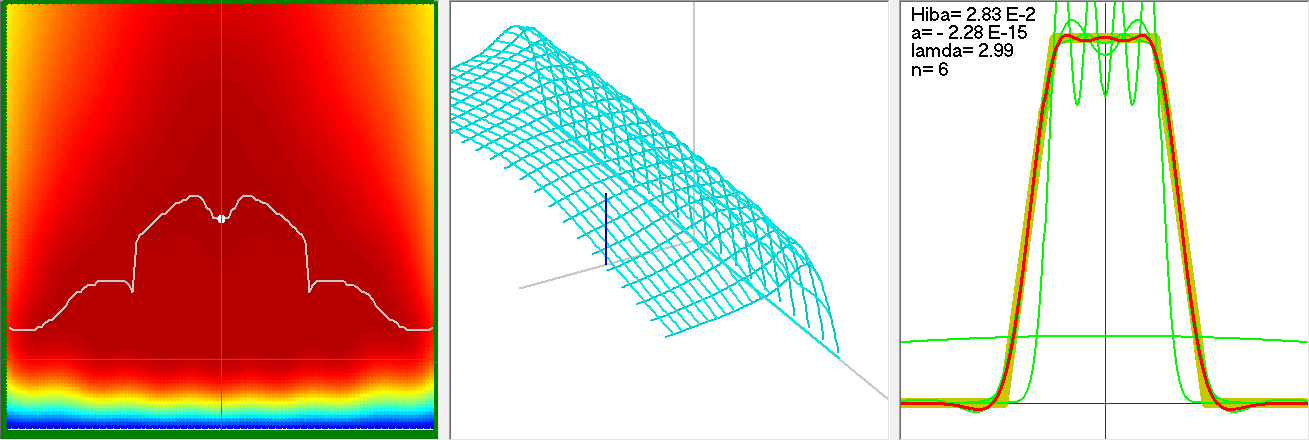
\includegraphics[width=140mm]{./Abrak/Ereszkedo1/Er36.png}
  \caption{Az $F_n$ által meghatározott felület, és approximáció}
\end{center}
\end{figure}

\section{A Nelder-Mead algoritmus}



A $Nelder-Mead$ szimplex algoritmust \cite{} eredetileg 1965-ben
fejlesztették ki azzal céllal, hogy létrehozzanak egy eljárást, amely
képes meghatározni egy $f : \Bbb R^n \to \Bbb R$ nemlineáris függvény minimum (maximum) helyét a  gradiens felhasználása  nélkül,
 pusztán a függvényértékekre  támszkodva. 
Mivel az algoritmust a bemutatott tömörítési eljárás során kétváltozós függvényekre kerül aklalmazásra, ezért ebben a speciális esetben szemléltetjük, megjegyezve, hogy hasonló 
elvek szerint
 működik az általános $n$ dimenziós eset is. Említendő továbbá, hogy Fejlesztői dokumentáció fejezetben bemutatott Nelder-Mead algoritmus implementációja képes kezelni az n-dimenziós esetet.  A minimum meghatározásához az $f(x_1), f(x_2), f(x_3)$  adnak kiindulási pontot, melyek közül egyet lecserélendő az adott lépésben. Nevezetesen, az algoritmus
\begin{equation*}
f(x_3)\le f(x_2)\le f(x_1)
\end{equation*}
 esetén olyan $x'$ helyet keres, amelyre $f(x')\le  f(x_3)\le f(x_2)$ teljesül és az $x_3, x_2, x_1$ ponthármasról az $x_1$-et elhagyva áttérünk az $x',x_3, x_2$ hármasra. Az $x'$ pontot az előzőekből geometriai transzformációkkal származtatjuk, felhasználva az  $x_2x_3$ szakasz $x=(x_2+x_3)/2$ felezéspontját: 
\begin{equation*}
x'=x_1+\alpha (x-x_1) \quad (\alpha\in\Bbb R)\,.
\end{equation*}
 Az alábbi ábrák szemléltetik az algoritmusban  használt transzformációkat. Látható, hogy $\alpha=2$ esetén $x'$ éppen az $x_1$ pont $x$-re vonatkozó középpontos tükrözése $(T_1).$ Továbbá $\alpha>2$ az eredeti háromszög tükrözése + nyújtása $(T_2),$ az $1<\alpha<2$ pedig tükrözéses + zsugorításnak felel meg $(T_3).$ A $-1<\alpha<0$ paraméterrel egyszerű zsugorítás adódik. Végül az 5. transzformáció $(T_5)$ az $x_3$ pontból történő
 kicsinyítésnek feleltethető meg. Az $x_1$ képe ezekben a transzformációkban és a hozzá tartozó függvényértékek a következő alakban adottak:
\begin{equation*}
x':=x_{3+i}=T_i(x_1)\quad (i=1,2,3,4), \qquad y_j=f(x_j)\quad (j=1,2,\cdots,7)\,.
\end{equation*}
Azt, hogy mikor melyik transzformáció használandó, a Függelékben, illetve a Fejlesztői dokumentáció Nelder-Mead algoritmus implementációjával foglalkozó fejezetben
található  folyamatábrából látható. Az említett műveleteket a \ref{fig:nmtrf} ábra szemlélteti.
\begin{figure}[htb!]
  \centering
\subfigure[Tükrözés\ $(T_1: \alpha=2).$]{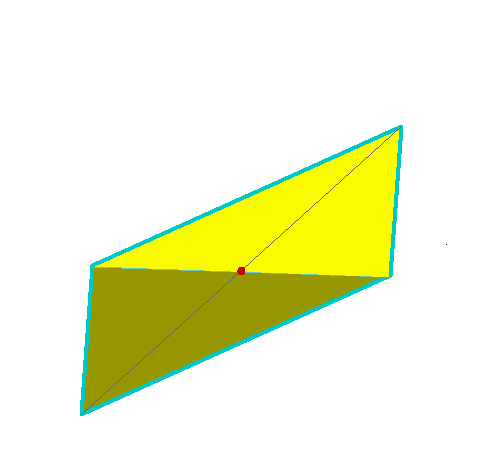
\includegraphics[scale=0.26,trim=10 0 10 53,clip]{./Abrak/Egyeb/NMT1.PNG}} 
\subfigure[T-Nyújtás\ $(T_2: \alpha=2.5).$]{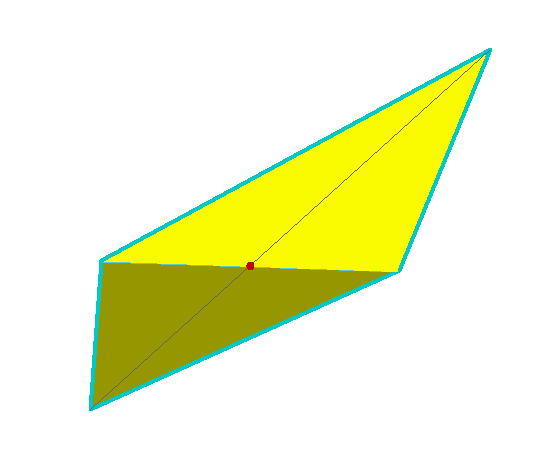
\includegraphics[scale=0.26,trim=10 0 10 53,clip]{./Abrak/Egyeb/NMT2.PNG}}
\subfigure[T-Összehúzás\  $(T_3:  \alpha=1.5).$]{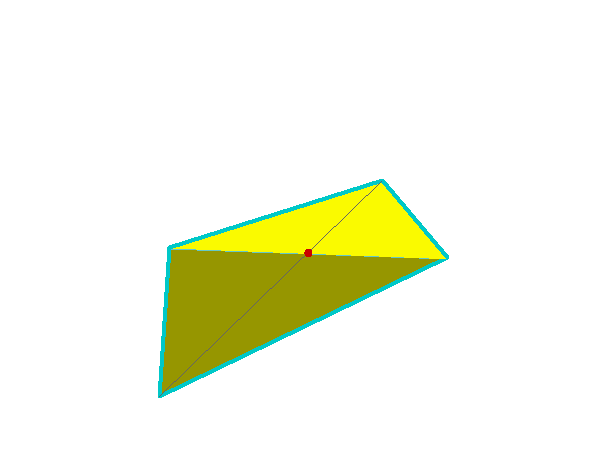
\includegraphics[scale=0.26,trim=10 0 10 53,clip]{./Abrak/Egyeb/NMT3.PNG}} 
\subfigure[Összehúzás\ $(T_4: -1<\alpha<0).$]{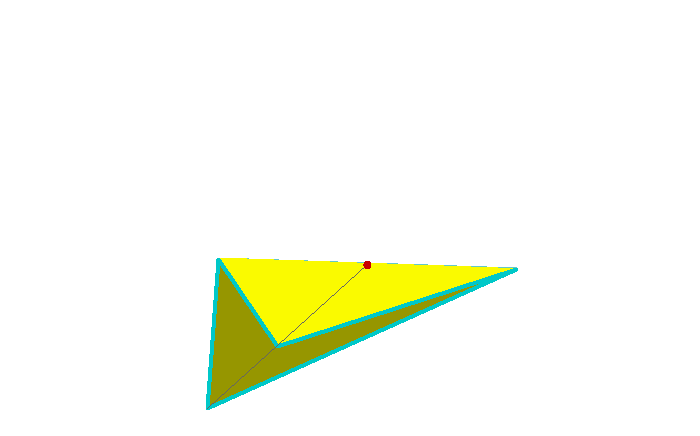
\includegraphics[scale=0.26,trim=10 0 10 185,clip]{./Abrak/Egyeb/NMT4.PNG}}
\subfigure[Kicsinyítés  $x_3$-ból $(T_5).$]{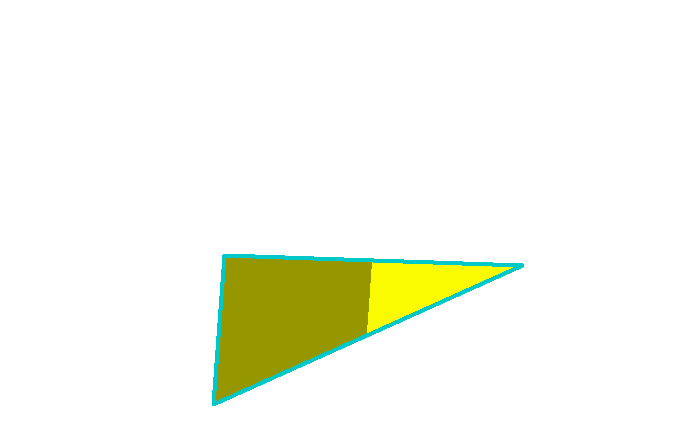
\includegraphics[scale=0.26,trim=10 0 10 185,clip]{./Abrak/Egyeb/NMT5.PNG}}
\caption{A $Nelder-Mead$ szimplex transzformációi.}
\label{fig:nmtrf}
\end{figure}

Megjegyezendő, hogy a $Nelder-Mead$ szimplex módszer egy determinisztikus algoritmus. Az algoritmus gyors, hiszen minden lépésben csak néhány függvénykiértékelést kell végezni. Továbbá, egyes módszerek, például a gradiens módszerrel ellentétben az olyan patologikus függvények optimumát is képes gyorsan megtalálni, mint amilyen a Rosenbrock függvény. 

\section{Kvadratúra formulák}


Mivel a $Nelder-Mead$ algoritmus
kizárólag a függvényértékekre támaszkodik, a hibafüggvény értékeinek kiszámításához elegendő az Hermite-függvényeket valamilyen felosztás pontjaiban egyszer meghatatározni. Ez implementációs szempontból is fontos, hiszen nem kell minden $(\lambda,a)$ paraméterhez kiszámolni az ettől függő, rekurzióval adott Hermite-féle függvényrendszer tagjait. Ehelyett elég az eredeti diszkrét adatsorozatot dilatálni, illetve eltolni, ami lényegesen kevesebb számítást igényel. Továbbá, az említett felosztás pontjainak valamely Hermite-függvény zérushelyeit választva, a hibafüggvényben  szereplő integrálok kiszámításához
a \cite{} dolgozatban használt eljáráshoz hasonlóan kvadratúra formulát is alkalmazhatunk. Ennek előnye, hogy az alappontokban a módszer interpolál, így itt lehetséges a jel mintáinak pontos rekonstrukciója. Ugyanakkor, a kapott approximáció is pontosabb, amit a \cite{}-ben közölt numerikus tesztek is alátámasztanak.
	\par Ahogyan ez a \cite{} dolgozatban látható, további optimalizációs algoritmusok is alkalmazhatóak a probléma megoldásához. Egy ezek közül a leggyosrabb ereszkedés módszere, melynek az alkalmazásához 
szükségünk van a függvény parciális deriváltjaira. Ezek előállításával ilyen esetben
külön  kell foglalkozni. Az Hermite-függvények deriváltjaira vonatkozó formulák alapján a
parciális deriváltakra a hibafüggvényhez hasonló ellőállítás adható. Ebben az esetben az \eqref{eq:dotprod} egyenletben szereplő integrálok kiszámításához ekvidisztans felosztása alkalmazandó.


\section{A tömörítő eljárás jellemzése}



A tömörítés kezdetekor az első feladat a teljes EKG mérést szívütésekre bontása. Ezt követően
az egyes szívütések a tömörítő eljárás bemeneti paramétereként válnak értelmezhetővé. Inicializálni kell továbbá
a tömörítő függvények által visszaadott, az aktuális szívütésre vonatkozó Fourier-együtthatókat, 
az approximáció hibáját, illetve az optimalizációs eljárások által meghatározott dilatációs és 
transzlációs paramétereket. \par
	
A tömörítés előkészítése nem ér véget a jel szívütésekre történő felbontásakor. A szívütéseket normalizálása is szükséges. Ez azt jelenti, hogy az első és utolsó helyen felvett értékeket összekötő egyenes, és az eredeti EKG különbségét tekinti az eljárás tömörítendő jelnek. Ezt az eljárást az irodalomban az alapvonal eliminálásnak nevezik. Ennek eredményeként a jel tartója a kezdő és a végpont által meghatározott intervallum. Végül, a szívütést normálásra kerül, vagyis az egyes értékeket 
elosztjuk az abszolút maximummal. \par
	A tömörítés megkezdése előtt inicializálni kell a függvényrendszert, 
melynek során az egyes bázisfüggvények által felvett értékek egy mátrix soraiba kerülnek: 
\begin{equation*}
	\Phi:=\left[\Phi_n(\alpha_m)\right]_{0\leq n < N,\;0\leq m < M}\,.
	\label{eq:phi_matrix}
\end{equation*}
A $\Phi\in\mathbb{R}^{N\times M}$ mátrix segítségével az $f\in\mathbb{R}^M$ diszkrét jel Fourier-együtthatói könnyen meghatározhatók:
\begin{equation*}
	c_n:=\left\langle f, \Phi_n \right\rangle=\frac{1}{M} \Lambda^{-1} \Phi f \quad (0\leq n < N)\,,
	\label{eq:phi_coeffs}
\end{equation*}
ahol $\mathbb{R}^{N\times N}\ni\Lambda=\Phi \Phi^T$ Cristoffel-Darboux számokat tartalmazza. Az előállításban szereplő $\alpha_n\in\mathbb{R}\, (0\leq n < N)$ számok a \ref{sec:kvad} fejezetnek megfelelően kétféleképpen határozhatóak meg. Egyrészt a $Nelder-Mead$ algoritmusban a $\Phi_N$ függvény gyökeit véve kvadratúra formulákat definiáltunk. Más optimalizációs algoritmusok, például a gradiens módszer esetén $f$ tartóján egyenletes alapponterndszert alkalmazandó. Figyelmet érdemel, hogy az előbbi esetben a gyökök pontos meghatározása kritikus a feladat szempontjából. A probléma megoldásához a \cite{gautschi} könyv által javasolt numerikus eljárás található az implementációban. Nevezetesen, a $H_n$ Hermite-polinom \eqref{eq:identities} rekurziójában szereplő együtthatókat egy tridiagonális mátrixba rendezzük. Könnyen belátható, hogy az $\alpha_n$ gyökök megegyeznek ezen tridiagonális mátrix sajátértékeivel.  \par

Hátra van még a megfelelő $(a,\lambda)$ paraméterek beállítása. Annak érdekében, hogy a reprezentáció minél adaptívabb legyen, több  optimális transzláció, illetve dilatáció meghatározása szükséges. Az eredeti $f\in\mathcal{F}$ jelet tehát a következő alakban közelíti a módszer:
\begin{equation*}
	S_{\mathbf{n}}^{\mathbf{a},\boldsymbol{\lambda}}f:=\sum_{i=1}^N\sum_{k=0}^{n_i} \langle f^{a_i,\lambda_i},\Phi_{k}\rangle\Phi_{k} \quad
	(a_k \in \Bbb R,\lambda_k>0)\,,
\end{equation*}
ahol $\mathbf{a}=a_1, a_2, \ldots, a_N$ az alkalmazott transzlációk, $\boldsymbol{\lambda}=\lambda_1, \lambda_2, \ldots, \lambda_N$ pedig a dilatációk sorozata. Az egyes sorfejtésekhez tartozó együtthatók számát az $\mathbf{n}=n_1, n_2, \ldots, n_N$ vektor jelöli. Mivel az EKG jel alapvetően három fő hullámból áll ezért jelen probléma megoldásakor $N=3.$ Továbbá a \cite{hexp3} dolgozat eredményei alapján
a QRS komplexumot egy heted, a T hullámot hatod, a P hullámot pedig egy másodfokú ortogonális rendszer segítségével approximálja az eljárás azaz $\mathbf{n}=7,6,2\,.$ Fontos, hogy a legjobb approximáció előállításához a \eqref{eq:hilaprx} egyenlettel ellentétben már az eredeti függvény $f^{a_i,\lambda_i}$ transzformáltja használatos. Ez nem jelent megszorítást az eredeti problémára nézve, implementációs szempontból viszont $f^{a_i,\lambda_i}$ kiszámítása gyorsabb, mint a $\Phi_n^{a_i,\lambda_i}$ rendszer előállítása.

A $(a_i,\lambda_i)$ paraméter párok optimalizációja egymástól függetlenül történik. Így azonban nem garantált, hogy az algoritmus a P, QRS, T hullámokat külön-külön approximálja. A problémát az irodalomban jól ismert ún. $Matching\ Pursuit$ $(MP)$ konstrukció \cite{mpurs} alkalmazásával oldja meg a módszer. Ez egy mohó algoritmus, mely minden lépésben a \eqref{eq:Fnfuggv} egyenletben definiált $F_n(a_i,\lambda_i)$ függvény maximalizálására törekszik. Az iteráció $i.$ lépése a következő alakban írható fel:
\begin{equation}
	s^{(i)}=s^{(i-1)} + S^{a_i,\lambda_i}_{n_i} R^{(i-1)} \quad (1\leq i \leq N)\,,
\label{eq:mpurs}
\end{equation}
ahol $R^{(i)}=f-s^{(i)}$ a rezidum függvényt jelöli. Röviden tehát az $s^{(0)}=0,\ R^{(0)}=f$ inicializálás után, az eljárás az $i.$ lépésében megkeresi az $R^{(i-1)}$ függvény $\ell^2$ norma szerinti legjobb közelítését, amit ki is von az említett rezidum vektorból. Ezt $N$ iteráción keresztül ismétli az aktuális $R^{(i)}$ függvényre. Az MP módszer egy gyors algoritmus, mellyel megkonstruálható az $f\in\mathcal{F}$ jel ritka reprezentációja. Emellett lehetséges az EKG szívütéseinek automatikus szeparációja is, hiszen a jel különböző részeit eltérő ortogonális rendszerek segítségével közelítjük. Figyelmet érdemel, hogy az eredeti \cite{hexp3} módszerben ezt a lépést egy külön szegmentáló algoritmus végezte. Így a közelítés pontossága erősen függött a szegmentálás eredményétől (lsd. \ref{sec:test} fejezet). A kifejlesztett eljárásnál azonban ez a probléma nem áll fenn még zajos jelek esetén sem. A dolgozatban bemutatott módszer iterációs lépéseit, az $R^{(i)}$ rezidum függvények alakulását, illetve a szeparált EKG jelet az \ref{fig:mpstep} ábra szemlélteti. Jól látható az is, hogy a fekete vonallal jelölt optimális transzláció általában nem az abszolút maximum helyén található. Ez indokolja, hogy a $\lambda_i$ dilatáció mellett az $a_i$ paraméter optimalizációjára is szükség van. Mivel ez utóbbi a kiindulásként használt \cite{hexp3} dolgozatból hiányzik, ezért a pontosság és tömörítési arány jelentős javulása várható el tőle.
\begin{figure}[htb!]
  \centering
\subfigure[A QRS approximációja.]{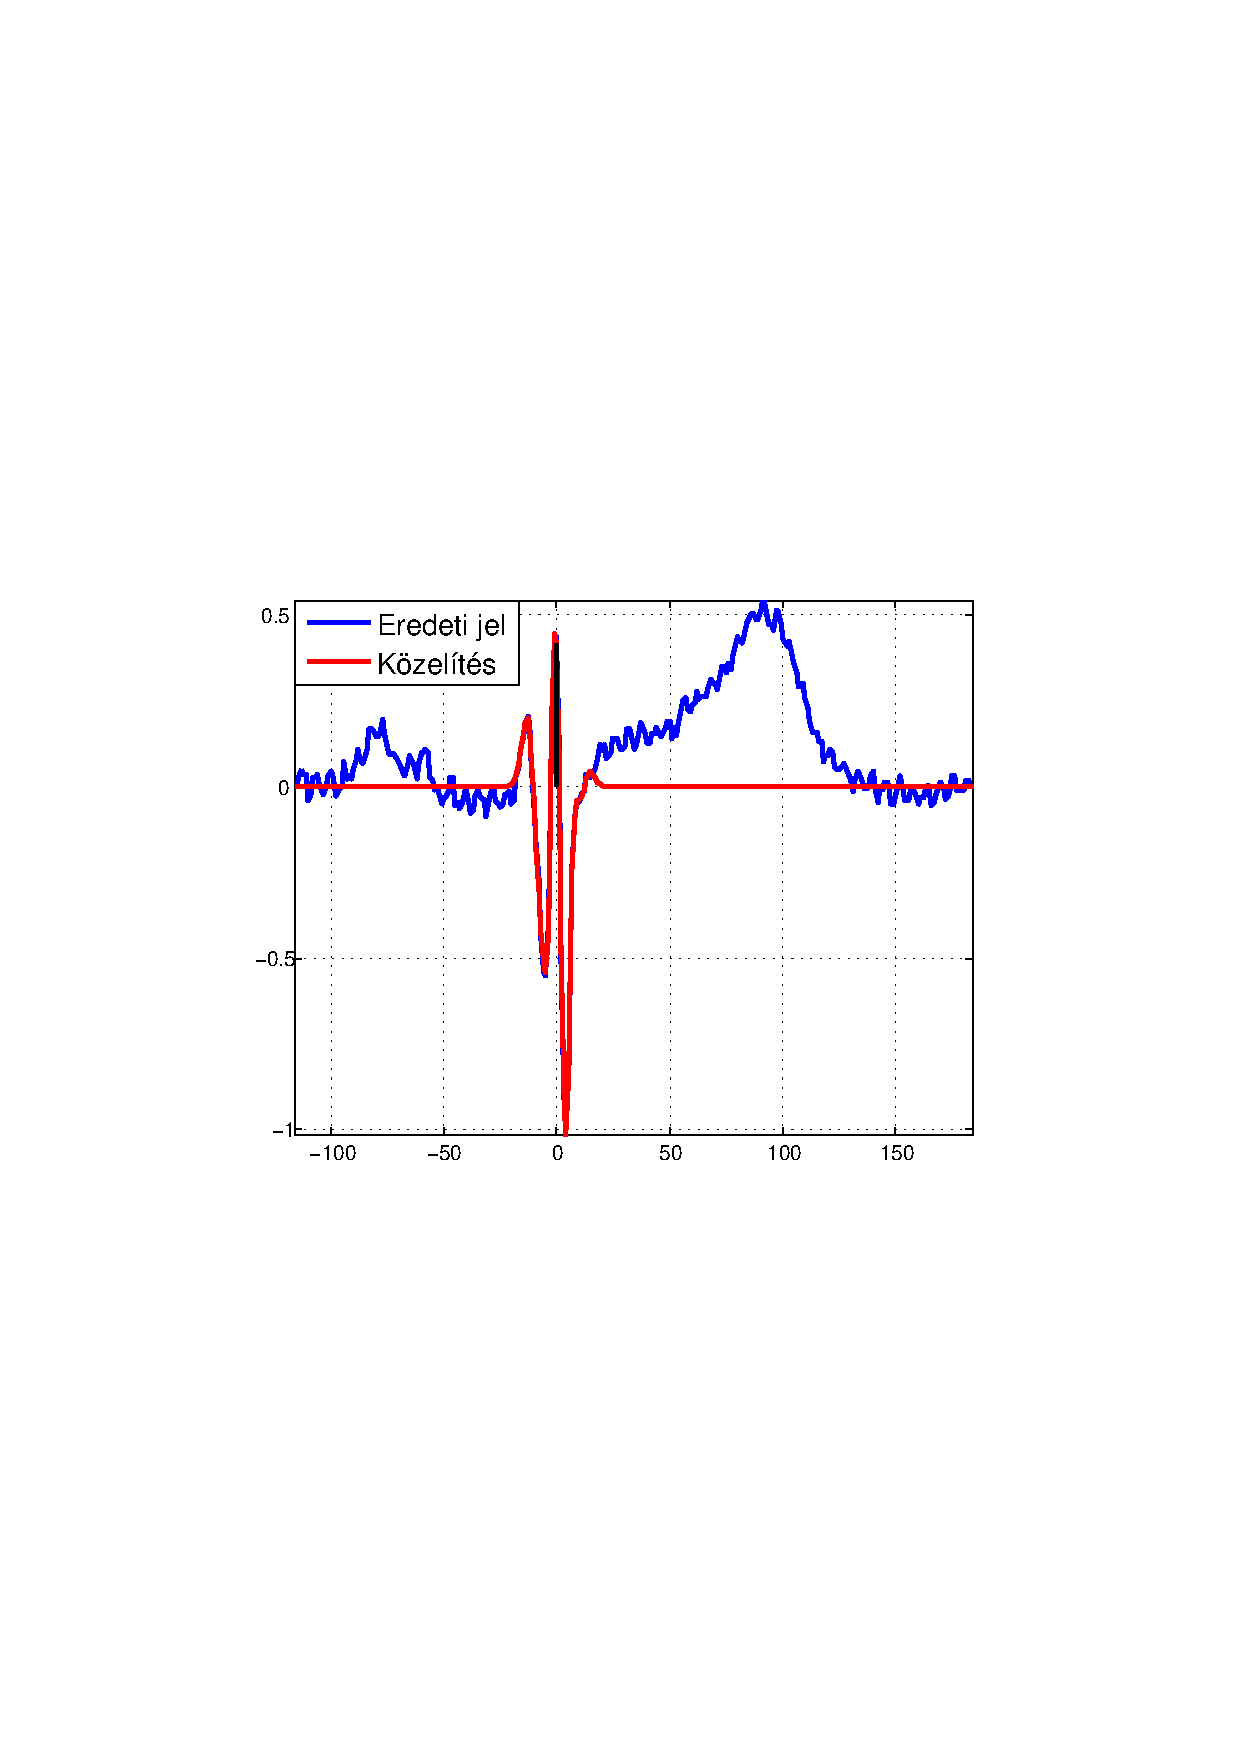
\includegraphics[scale=0.5,trim=120 280 100 280,clip]{./Abrak/Lepesek/abra_lepes0.pdf}} 
\subfigure[A T hullám approximációja.]{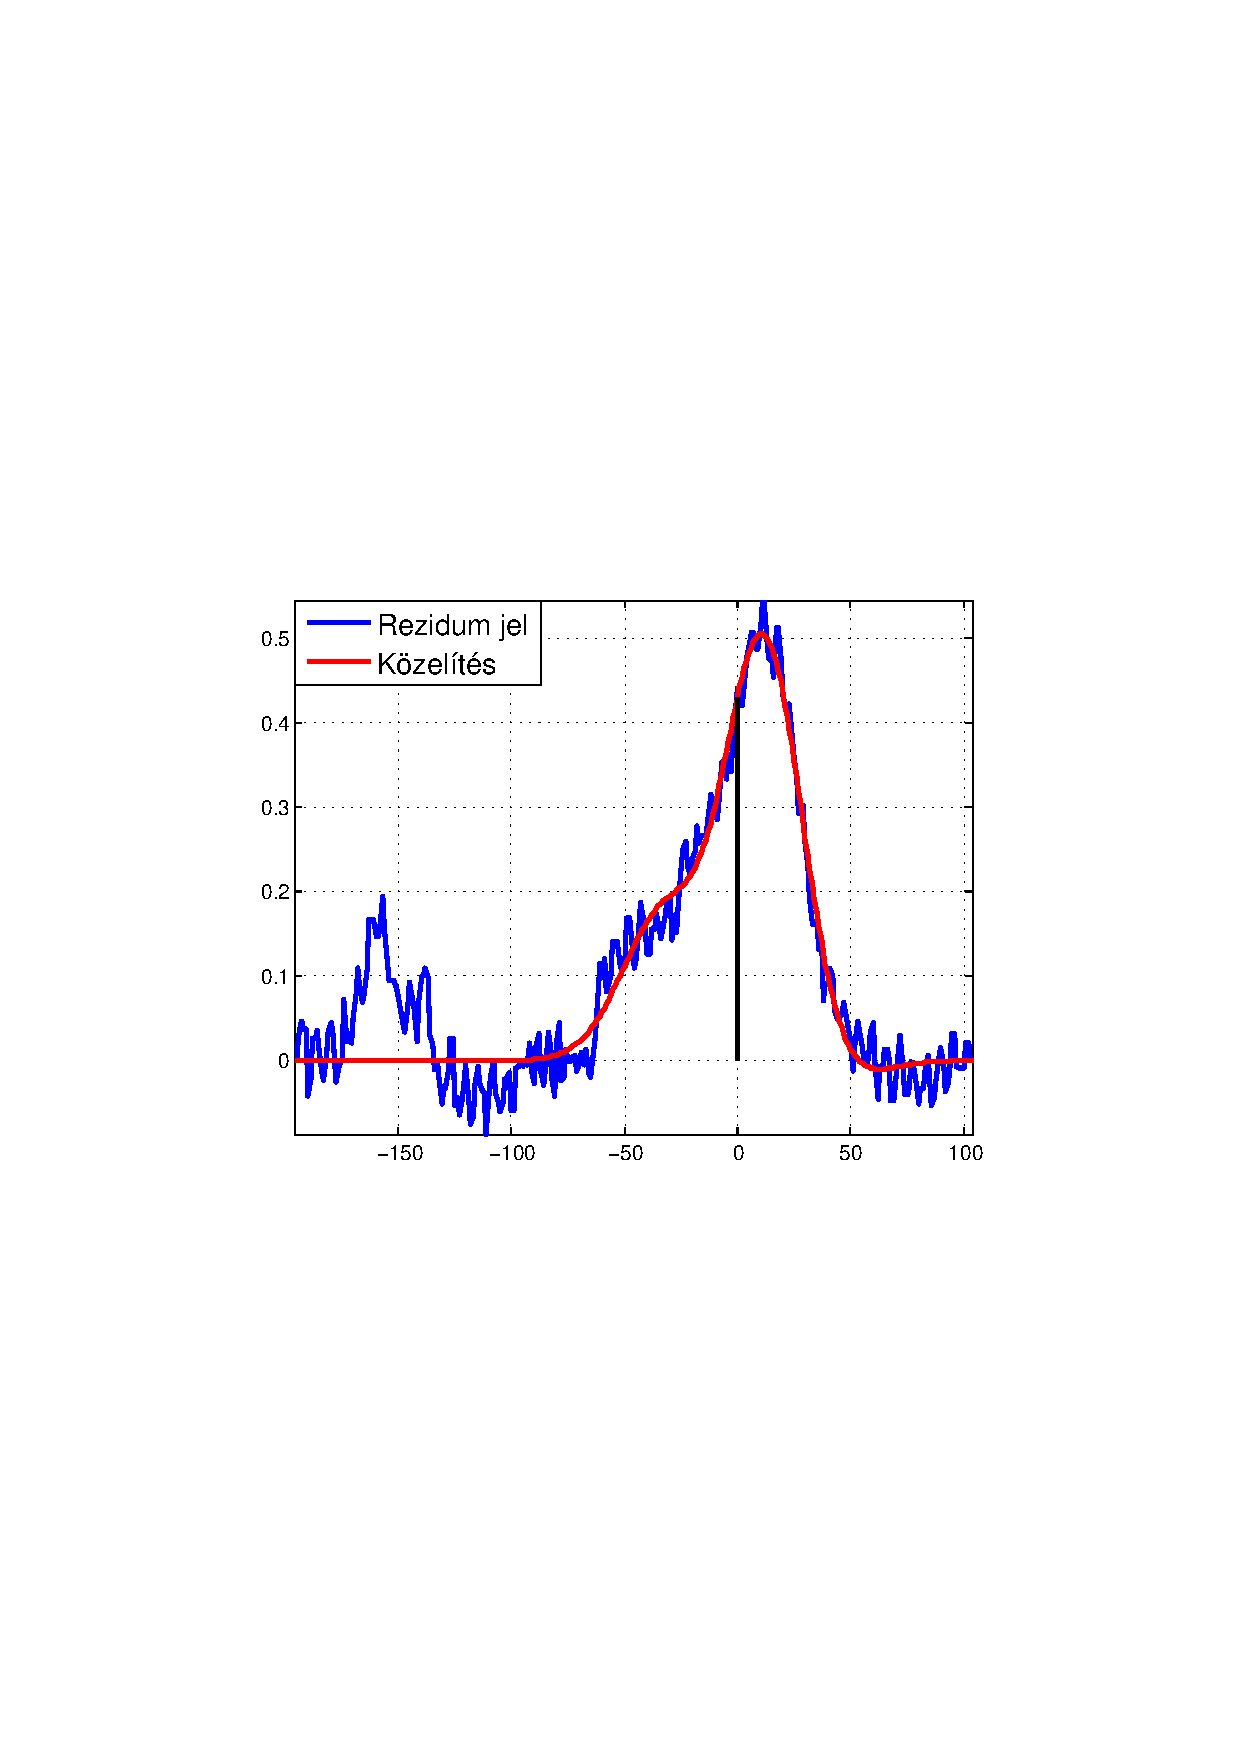
\includegraphics[scale=0.5,trim=120 280 100 280,clip]{./Abrak/Lepesek/abra_lepes1.pdf}}
\subfigure[A P hullám approximációja.]{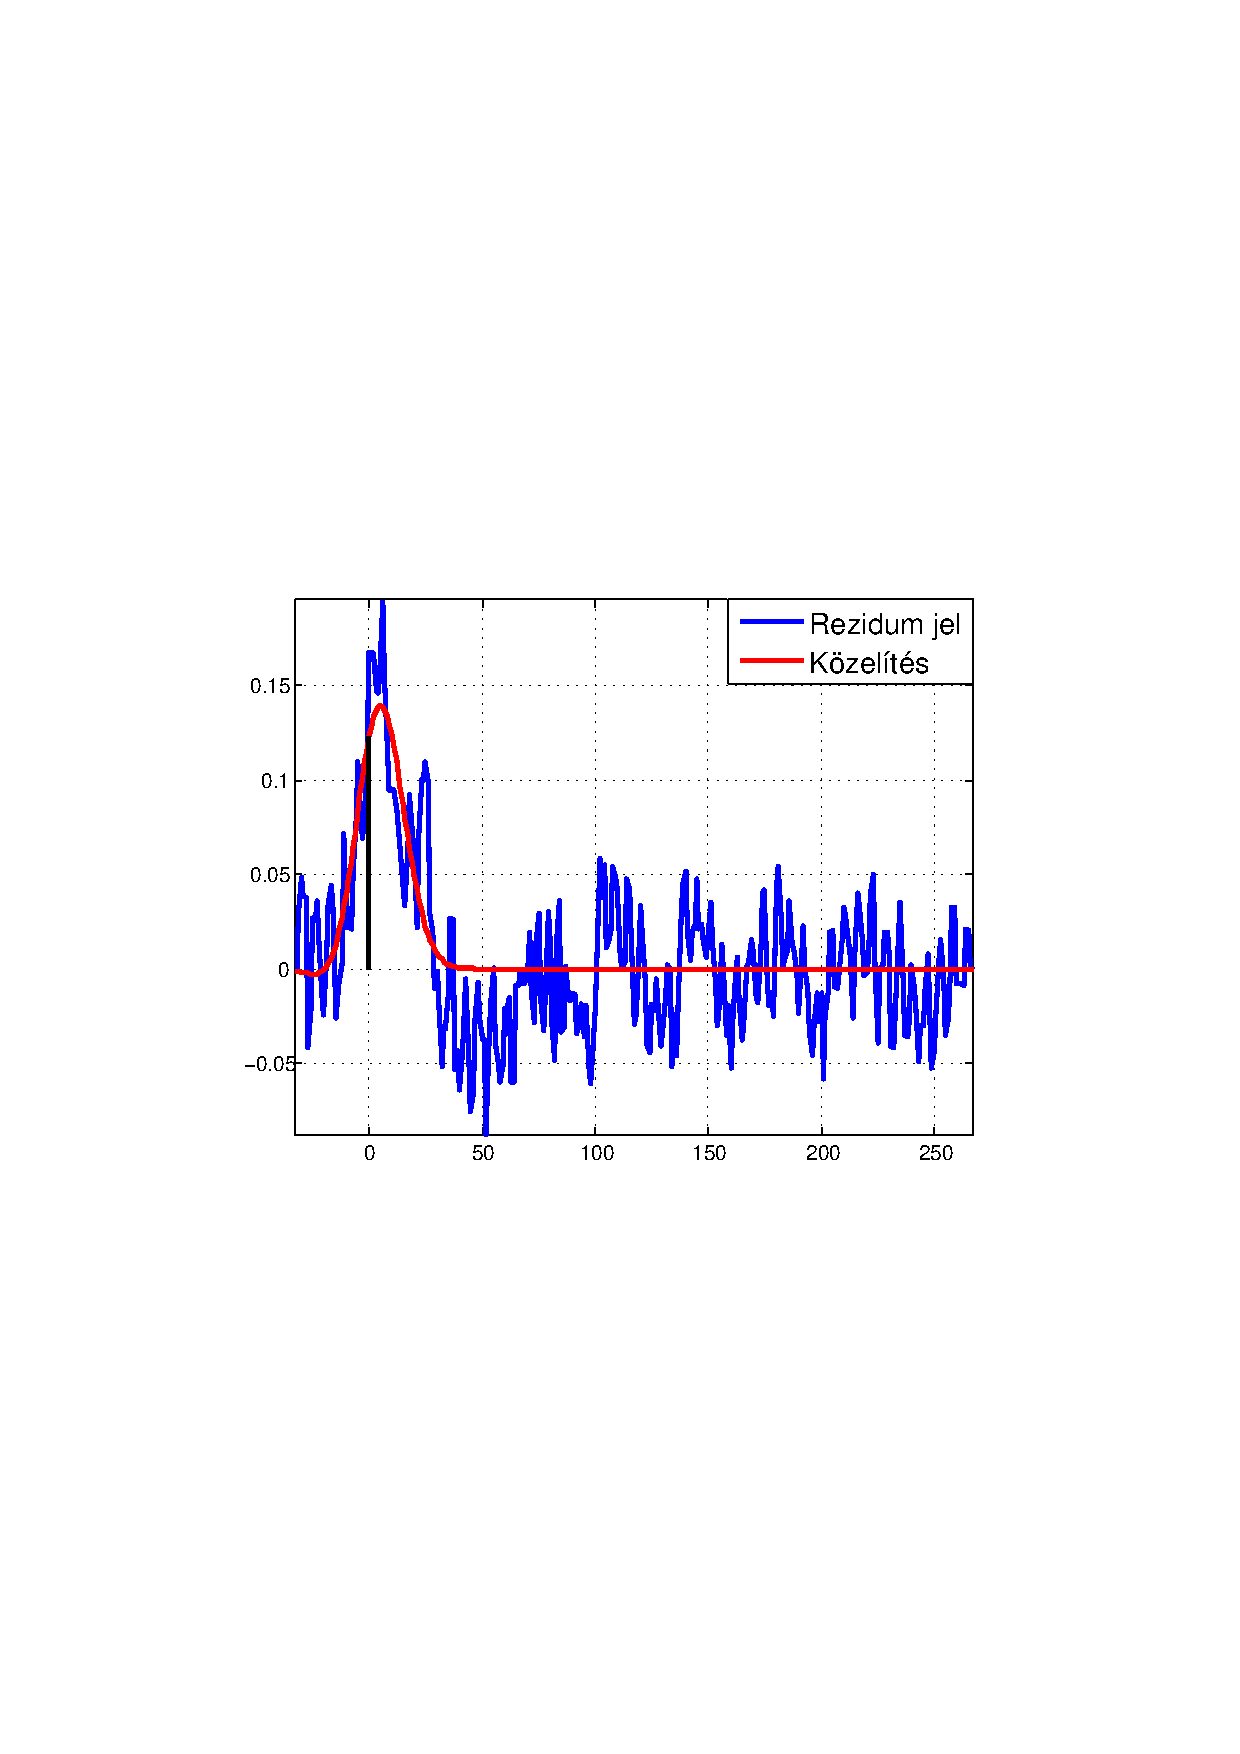
\includegraphics[scale=0.5,trim=120 280 100 280,clip]{./Abrak/Lepesek/abra_lepes2.pdf}} 
\subfigure[Szeparált szívütés.]{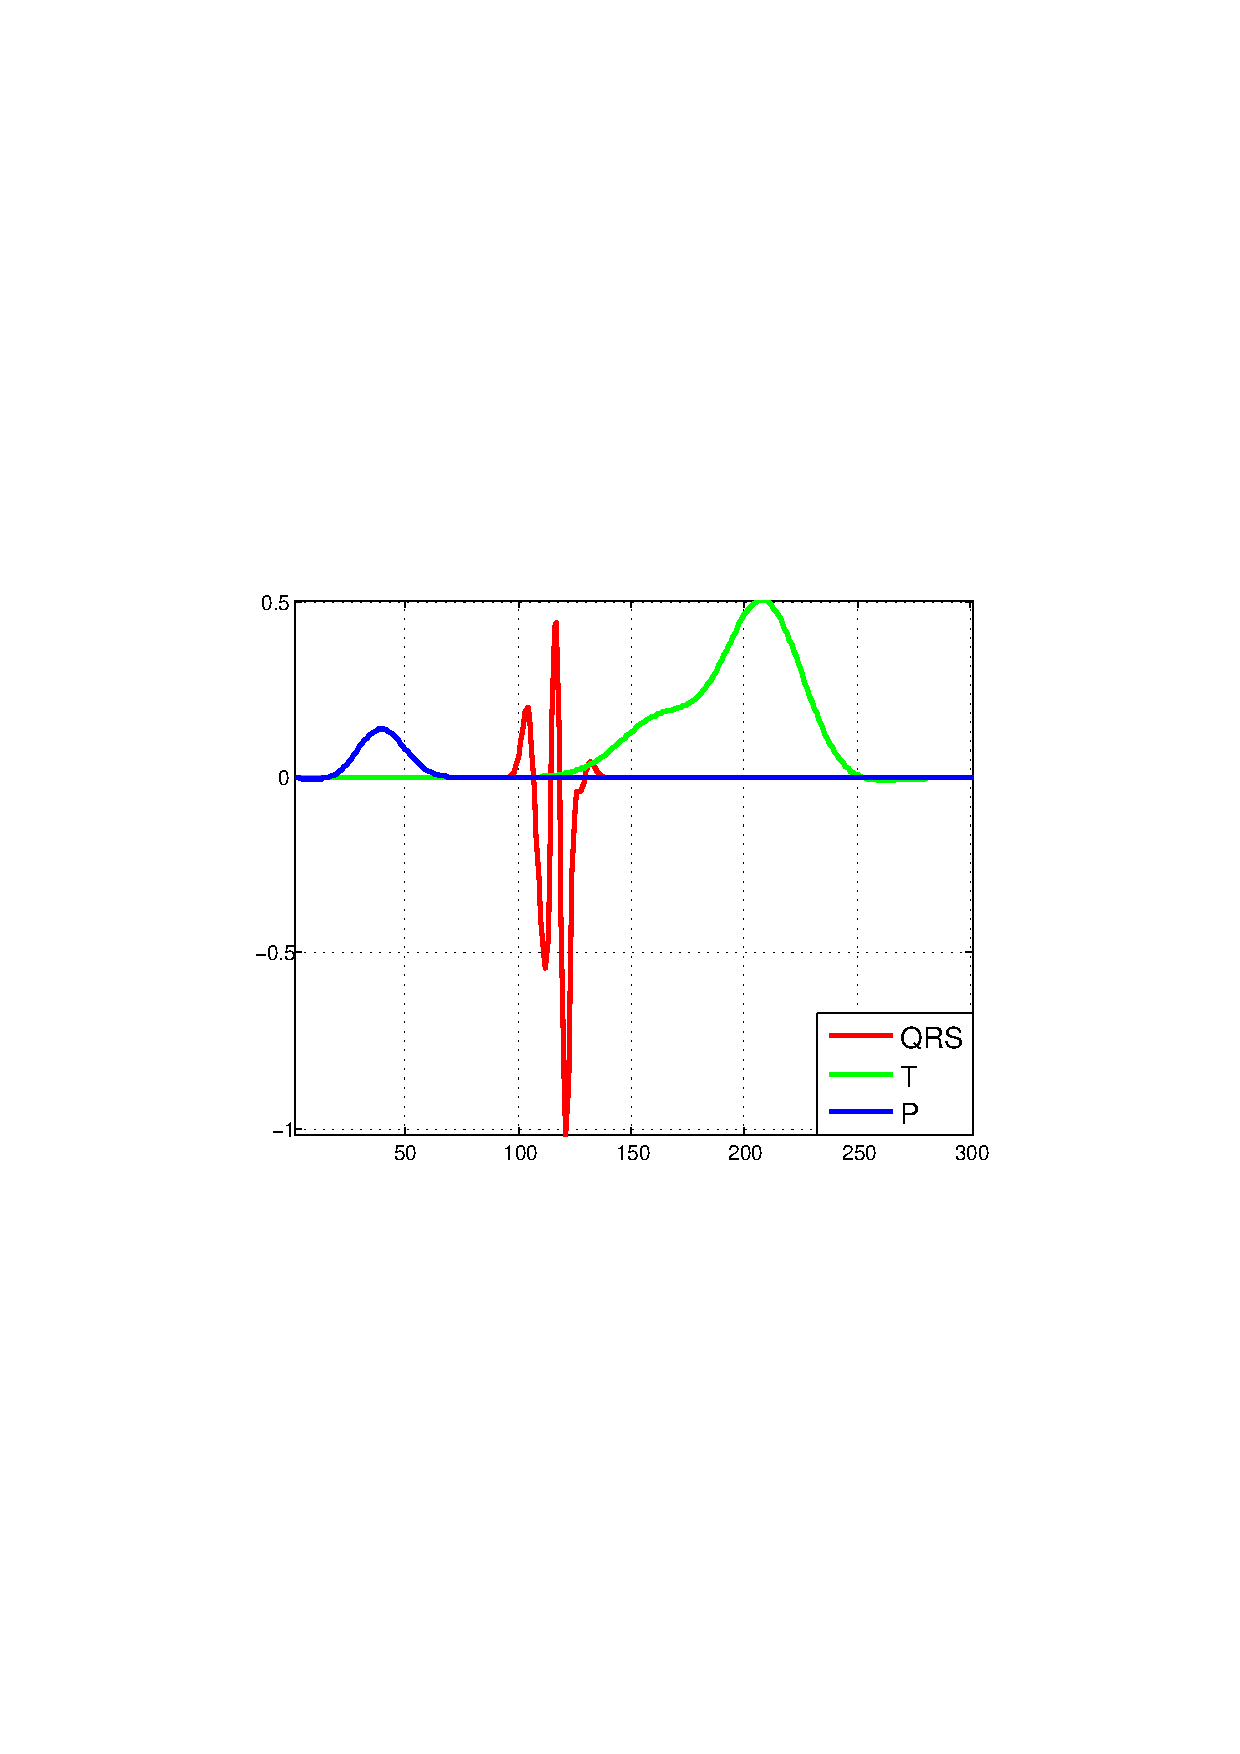
\includegraphics[scale=0.5,trim=120 280 100 280,clip]{./Abrak/Lepesek/abra_lepes3.pdf}}
\caption{Az MP algoritmus lépései.}
\label{fig:mpstep}
\end{figure}


\chapter{Felhasználói dokumentáció}

\chapter{Fejlesztői dokumentáció}

Ebben a fejezetben található a Bevezetés-ben bemutatott eljárás implementációjának pontos (modul szintű) leírása, valamint az alkalmazott tesztek jellemzése illetve ezek eredményei. A tesztelés eredményeit a tapasztalok összegzése és néhány lehetséges jövőbeli fejlesztés jellemzése követi. \par A fejlesztői dokumentáció első részében a tömörítési módszer implementációjának leírása található. Ez az alfejezet két fő részre tagolható: a webes felhasználói felület és az ehhez felhasznált könyvtárakat leíró, valamint a háttérben a konkrét tömörítést elvégző c++ program modulonkénti jellemzését. Mivel a webes felület megvalósítása rövid, és specializált scriptek összessége, ezért ezek jellemzését minden esetben egyedi módon érdemes kezelni. Ellentétben ezzel a szemlélettel, a c++ program nagyban épít a nyelv által támogatott objektum orientált megközelítésre. Ez lehetővé teszi és indokolja is egyben, hogy az implementációt jellemző dokumentáció is hasonlóan jól strukturált legyen. Az egyes modulok dokumentációja ugyanazon három szempont szerint közelíti meg a jellemzésüket: a modul feladatának, a modul interfészének (hogyan és mely egyéb modulokhoz kapcsolódik), valamint a modult felépítő osztályok implementációjának pontos megfogalmazása. A modulok leírásánál találhatóak továbbá a szemléltetést segítő UML és egyéb hasznos diagrammok. 
\par  A teszteléssel foglalkozó alfejezet szintén több részre tagolható. Az első alfelejezetben található a webes felhasználói felület funkcióinak tesztelési terve, illetve az egyes tesztek eredményeinek leírása. Ezt követi a c++ program moduljainak részletes tesztelési terve. A modulok tesztelését minden esetben egy külön tesztfájl végezte. Ennek leírása, az eredmények értékelése, illetve a tesztállomány elérési útja szintén megtalálható az alfejezetben. A  tesztelés alfejezet utolsó része a bemutatott tömörítési eljárást hivatott tesztelni. Ez több szempont alapján, egyéb EKG tömörítő módszerekkel történő összehasonlítás útján valósul meg. A tesztek eredményeinek jellemzését az egyes elfajuló, különleges esetek közelebbi vizsgálata, majd egy rövid kitekintés követi.

\section{A felhasználói felület implementációja}

\section{A tömörítő eljárás implementációja}

A felhasználói dokumentáció bevezetésében leírtakkal összhangban, a tömörítő eljárás implementációjával foglalkozó fejezet minden pontja három részre tagolható. Minden alfejezet az aktuális modul feladatának pontos megfogalmazásával kezdődik. Ezt követi a modul interfészének definiálása, melynek segítségével átlátható a modul kapcsolata a program többi részével. Végül a modult alkotó osztályok és strukturák fő metódusainak, illetve adattagjainak leírása következik. A program robosztussága indokolja, hogy minden egyes metódus és függvény ne kerüljön itt jellemzésre, azonban a program forráskódjában minden metódus előtt megtalálható annak rövid jellemzése, elvárt bemenete, és esetleges visszaadott értékének típusa. Az egyes modulok dokumentációja tartalmazza ezen kívűl az ezeket leíró UML, és egyéb diagrammokat. Az egyes modulok imlpementációja külön .h, és .cpp kiterjesztésű állományokban található, ezért az egyes alfejezetek címei megegyeznek ezen állományok elnevezésével. A fejezet utolsó alfejezete leírást biztosít az implementáció által felhasznált külső könyvtárakhoz, illetve indokolja ezek választását.

\subsection{A SigPrep modul implementációja}

Az implementációt tartalmazó mappaszerkezet gyökerét \texttt{/}-vel jelölve, a SigPrep modult  az \texttt{/src/headers/SigPrep.h}, illetve az \texttt{/src/SigPrep.cpp} állományok implementálják. \par A modul feladata, hogy egységes módszert biztosítson a bemeneti jelek kezeléséhez. 
Mivel az eljárás EKG jelek tömörítésével foglalkozik, illetve speciálisan az MIT-BIH adatbázisban megtalálható egyedi formátumú jelek feldolgozásával, 
ezért egy általános jel kezelő modul implementációja nem volt szükséges a módszer megvalósításához. Annak érdekében azonban, hogy 
hogy a bemutatott jel tömörítő eljárást jövőbeli vizsgálódások során könnyen ki lehessen próbálni egyéb jel típusokon, fontos az ehhez szükséges, általános metódusok definiálása. A SigPrep modul feladata tehát, hogy definiálja azokat az egységes függvényeket amelyek elengedhetetlenek a bemeneti jelek programon belül történő kezeléséhez. Ezen kezelési módszerek pontos megvalósítását a \texttt{/src/headers/SigPrep.h} állományban található SigPrep osztályból származtatatott osztályok, (a jelenlegi programcsomagban a \texttt{EcgSigPrep} osztály), írják le. 
\par A SigPrep modul közvetlenül nem kerül példányosításra a feladat megoldásának érdekében. Külső szolgáltatásokat a modul nem vesz igénybe a programcsomag egyéb elemeitől, azonban az általa definiált metódusokra erősen támaszkodik a \texttt{SigPrep} osztályból származtatott \texttt{EcgSigPrep} osztály. A SigPrep modul legfontosabb szolgáltatása a belőle származtatott osztályok felé, hogy pontosan meghatározza egy tömöríthető jel formáját és elemeit. További szolgáltatásként a modul biztosítja az átírható (virtuális) \texttt{virtual void SigPrep::setSignal()} metódust a jel éppen tömöríteni kívánt részének inicializásához. Az eddig felsoroltakon kívül a SigPrep modul getter függvényeket definiál a teljes tömörítendő jel (például sok órányi EKG jel), az éppen tömörítendő jel részlet (egyetlen szívütés), illetve ennek bizonyos szignifikáns értékeihez. 
\par A SigPrep modult kizárókag a \texttt{SigPrep} osztály alkotja. Összesen öt protected hozzáférhetőségű adattaggal rendelkezik. Ezek közül kettő \texttt{Eigen::MatrixXd} mátrix típusra mutató pointer, melyek feladata a tömörítendő jelhez való hozzáférés biztosítása. Az \texttt{entire\_signal} azonosítójú mutatón keresztül lesz képes a \texttt{SigPrep} osztály elérni a teljes EKG mérést. A második mutató a \texttt{signal} azonosítóval van ellátva, és a teljes mérésen belül egy-egy szívütéshez való hozzáférést biztosítja. Ennek megadása fontos, mivel egy EKG mérés jellemzően sok szívütésből áll a bemutatott tömörítési eljárás pedig szívütésenként alkalmazható. A mutatókon kívül még három protected hozzáférhetőségű, \texttt{double} adattagot definiál a \texttt{SigPrep} osztály. Ezek rendre a \texttt{sig\_first\_val, sig\_last\_val}, illetve \texttt{sig\_max\_val} azonosítókkal vannak ellátva. Ezek az adattagok tárolják az aktuális, tömörítendő szívütés értékeit az eredeti jel első, utolsó és legnagyobb abszolút értékű pontjában. Erre az információra abban az esetben lehet szükség, ha a kitömörített jelet a méréssel azonos formára kell hozni, ugyanis magát a tömörítést egy "normált" jelen végzi a program. Ennek a "normálásnak" egy lehetséges megvalósítását implementálja a szintén protected hozzáférhetőségű \texttt{virtual void setSignal()} metódus. A metódusnak két fontos feladata van: az eredeti szívütésből kivonni az első és utolsó pontját összekötő egyenest, ezáltal eltávolítva a szívütésben található "baseline wandert" \ref{ekg konyv}, valamint elosztani a jel összes értékét a legnagyobb abszolút értékű elemével. Ez transzformáció lehetővé teszi a szívütések pontosabb közelítését olyan ortogonális függvényrendszerek segítségével (mint például az Hermite függvények), amelyek gyorsan tartanak a 0-hoz, ha $|x| \to \infty$. Természetesen a \texttt{setSignal()} definíciója nem jelent optimális előkészítést minden lehetséges tömörítési eljárás esetén, ezért a metódust \texttt{virtual}-ként deklarálja a \texttt{SigPrep} osztály. Ez lehetővé teszi, hogy a \texttt{SigPrep} osztályból származtatott jelkezelő osztályok felüldefiniálhassák a \texttt{setSignal()} metódust. 
\par A \texttt{SigPrep} osztály konstruktorának egyetlen feladata, hogy a dinamikus memóriában helyet foglaljon a \texttt{signal} és az \texttt{entire\_signal} pointerek által mutatott mátrixoknak. Az osztály destruktora ezeket a címeket szabadítja fel.  Ezeken kívül összesen öt publikus hozzáférhetőségű függvényt definiál. \linebreak A \texttt{const Eigen::MatrixXd*} \texttt{getSignal()}, illetve a \texttt{const Eigen::MatrixXd*} \linebreak \texttt{getEntireSignal()} konstans mutatótak adnak vissza, melyek rendre a \texttt{signal} és az \texttt{entire\_signal} adattagokra mutatnak. Ezek a függvények lehetővé teszik az objektum által feldolgozni kívánt jel megismerését más modulok számára, azonban ezen a jelen változtatásokat kizárólag a \texttt{SigPrep}, illetve az ebből származtatott osztályok végezhetnek.
\par Az osztály további publikus függvényei konstans \texttt{double} értékeket adnak vissza, és a \texttt{const double getSigFirstVal()}, \texttt{const double getSigLastVal()} illetve \texttt{const double getSigMaxVal()} szignatúrák által azonosíthatók. Ezek a függvények a protected hozzáférhetőségű \texttt{virtual void setSignal()} függvény által megváltoztatott jel értékek lekérdezésére képesek. Ugyan a programcsomag jelenleg nem használja fel őket, a helyreállított (kitömörített) jel eredeti formára hozásánál lenne alkalmazható az általuk biztosított szolgáltatás.   


\subsection{Az EcgSigPrep modul implementációja}

Az implementációt tartalmazó mappaszerkezet gyökerét \texttt{/}-vel jelölve, az EcgSigPrep modult  az \texttt{/src/headers/EcgSigPrep.h}, illetve az \texttt{/src/EcgSigPrep.cpp} állományok implementálják. 
\par A modul feladata, hogy definiálja azokat a függvényeket és metódusokat amelyek az MIT-BIH EKG jel adatbázisban található méréseket egy Hermite függvény rendszer segítségével tömöríthető állapotba hozzák. A modul célja, hogy a fennt említett adatbázisban szereplő bármely mérés azonosítóját kapva bemenetül, a mérésben szereplő, tömörítendő elvezetést egy mátrixos alakban adja meg. A feladat részét képezi továbbá, hogy a modul képes legyen az így megadott jel összehúzására és eltolására különböző dilatációs és transzlációs adatok esetén. Összefoglalva tehát a modul legfőbb feladata, hogy Hermite függvényekkel történő tömörítés esetén a bemeneti EKG jeleket kezelhető állapotba alakítsa, illetve szükség esetén manipulálja őket.  
\par Az EcgSigPrep modult a \texttt{/src/headers/EcgSigPrep.h} állományban deklarált \texttt{EcgSigPrep} osztály alkotja. Az \texttt{EcgSigPrep} osztály a \texttt{SigPrep} osztályból lett származtatva, így birtokolja annak minden protected, illetve publikus hozzáférhetőségű adattagját és függvényét. Ez egyben úgy is értelmezhető, hogy az EcgSigPrep modul közvetlenül igénybe veszi a SigPrep modul szolgáltatásait. Az EcgSigPrep modul a feladatának megfelelően az MIT-BIH EKG adatbázisban található jelek ábrázolásához és manipulálásához biztosít szolgáltatásokat. Ezeket közvetlenül a MatchingPursuit modul veszi igénybe, a MatchingPursuit modulon keresztül pedig az EcgSigPrep osztályból példányosított objektumok által kiszámított jel értékekre támaszkodnak az OrtCompresser és NelderMead osztályok szolgáltatásai. 
\par Az \texttt{EcgSigPrep} osztály a \texttt{SigPrep} osztálytól megörökölteken kívül további négy protected hozzáférhetőségű adattagot definiál. Az \texttt{std::queue<WFDB\_Annotation> annotations} adattag tárolja az adatbázisból letöltött jelhez tartozó annotációkat (az EKG jel orvosok által megjelölt nevezetes pontjait), olyan sorrendben ahogyan azok a mérésben szerepelnek. A jelenlegi implementáció ezeket az annotációkat kizárólag az EKG mérés szívütésekre bontásához alkalmazza, azonban későbbi fejlesztések (például osztályozás implementációja) felhasználhatnák ezeket az adatokat ellenőrző értékek gyanánt. A \texttt{curr\_pos} egész típusú adattag hivatott tárolni a mérés tömörítésekor az éppen aktuális szívütés sorszámát. A \texttt{dilat}, illetve \texttt{trans} azonosítójú adattagok a jel összehúzásának illetve eltolásának mértékét tárolják. Ezek rendre \texttt{double}, illetve \texttt{int} típusúak. A transzlációs paramétert egész típusúnak definiálja az \texttt{EcgSigPrep} osztály, mivel az eltolást a jelet tartalmazó mátrix ( $ signal \in \Bbb R^{1 \times n} $ ) indexein definiálja. A \texttt{SigPrep} osztálytól megöröklt \texttt{virtual void SigPrep::setSignal()} metódus definícióján az \texttt{EcgSigPrep} osztály nem változtat, illetve ezen kívül egyéb protected hozzáférhetőségű függvényt nem definiál.
\par Az \texttt{EcgSigPrep} osztály konstruktora bemeneti paraméterként a feldolgozandó EKG mérés azonosítóját, a mérésben található elvezetések számát, illetve a mérést alkotó mintavételi pontok számát várja. Utóbbi paramétert önkényesen megválasztva lehetséges a teljes mérés helyett annak mindössze egy részét feldolgozni. A konstruktor két fő feladata, hogy a mérésekben szereplő értékeket a \texttt{signal} illetve \texttt{entire\_signal} pointerek által mutatott memória területre másolja, illetve feltöltse az \texttt{annotations} sort az egymást követő QRS komplexumot jelölő minták sorszámaival. Ezen feladatok elvégzésének érdekében a konstruktor felhasznája a \texttt{wfdb}, EKG mérés kezelő külső könyvtár függvényeit és típusait. A könyvtár dokumentációjáról, illetve főbb jellemzőiről a \ref{Külső könyvtárak} alfejezet értekezik. Miután az EKG mérés beolvasásra került, illetve az \texttt{annotations} sor feltöltődött a megfelelő pozíciókkal, a konstruktor meghívja az \texttt{EcgSigPrep::getNextSegment()} függvényt, ezzel biztosítva, hogy a \texttt{signal} pointer által mutatott területre a mérésben szereplő legelső szívütés minái kerülnek. Az \texttt{EcgSigPrep} osztály nem definiálja felül, illetve nem egészíti ki a \texttt{SigPrep} osztályban implementált destruktort. 


\par A konstruktoron és a destruktoron, valamint a 
\texttt{SigPrep} osztálytól megörökölt publikus hozzáférhetőségű függvényeken kívül az
\texttt{EcgSigPrep} osztály további négy publikus metódust definiál. Az első ezek közül a konstruktor által is igénybe vett 
\texttt{const Eigen::MatrixXd* getNextSegment()} 
szignatúrával elátott függvény. Ennek a függvénynek a feladata, hogy a feldolgozás során, a mérésben soron következő szívütés mintáit a \texttt{signal} pointer által mutatott memória területre másolja. A megvalósítás először ellenőrzi, hogy található-e még fel nem dolgozott szívütés az 
\texttt{entire\_signal} pointer által mutatott, teljes mérést tartalmazó mátrixban. Amennyiben igen, az \texttt{annotations} sorból egy \texttt{pop()} 
művelet segítségével a következő R csúcsot tartalmazó annotáció kivételre kerül. A \ref{QRS hermite cikk} tanulmányban írtak szerint a szívütés végét az így kapott R csúcstól számított következő 150 minta jelenti. Amennyiben ez a szám meghaladná a mérésben található minták számát,úgy a függvény a mérésben található utolsó mintát tekinti a szívütés végének. A függvény a \texttt{curr\_pos}, és a szívütés vége között található mintákat az \texttt{entire\_signal} által mutatott mátrixból a \texttt{signal} pointer által mutatott mátrixba másolja át. Ezt követően a függvény a jelenlegi mérésbeli pozíció, a \texttt{curr\_pos} adattag értékét lecseréli a szívütés utolsó mintájának indexére. Végül a függvény meghívja a \texttt{SigPrep::setSignal()} \ref{SigPrepmodul leírása} metódust, amely normalizálja  a szívütést, majd visszaad egy a \texttt{signal} pointerrel megegyező konstans mutatót. 
\par  Az \texttt{EcgSigPrep} osztály publikus függvényeként definiált \texttt{Eigen::MatrixXd} \linebreak \texttt{setDilatTrans(const double \&l, const double \&t, const Eigen::MatrixXd*} \linebreak \texttt{alpha, Eigen::MatrixXd\& sig)} szignatúrával ellátott metódus felel a paraméterként kapott dilatáció illetve transzláció a szintén bemeneti paraméterként kapott szívütésen történő alkalmazásáért. A függvény \texttt{alpha} azonosítóval ellátott paramétere egy magas fokú Hermite függvény zérushelyeit tartalmazó mátrixra ( $ alpha \in \Bbb R^{1*n} $ ) mutató pointer. A \texttt{setDilatTans} függvény először meggyőződik róla, hogy a paraméterként kapott dilatáció nullától eltérő értékkel bír. Amennyiben a dilatáció értéke nulla, a függvény ezt 1-re változtatja. Ezt követően a paraméterként kapott transzlációs értéket egész értékké alakítja. Miután kiszámította a végleges dilatációs és a transzlációs értékeket, a függvény definiálja az X,Y n elemű \texttt{std::vector<double>} típusú adatszerkezeteket, valamint az \texttt{ArrayXd} típusú \texttt{domain} azonosítóval ellátott, 0-ra szimmetrikus n elemű, egyenletes felosztású intervallumot, ahol n a szívütésben szereplő minták számát jelöli. Az \texttt{X} vektorba kerülnek a \texttt{domain} tömb dilatációval megszorzott elemei. Ez maga az "összehúzott" intervallum, amely fölött a függvény a jelet értelmezni fogja. Az Y vektor először a \texttt{sig} azonosítóval ellátott bemeneti jel elemeit kapja értékül. Az eltolás az Y vektor elemein alkalmazott \texttt{std::rotate} standard library-ban található függvény segítségével valósul meg. Ezt követően a \texttt{setDilatTrans} függvény a \texttt{Spline.h} külső állomány segítségével definiál egy spline-t, amely Y értékeit az X pontjaiban interpolálja. Az összehúzott és eltolt jel értékei megegyeznek az interpolációs spline értékeivel abban az esetben, ha annak az éppen vizsgált pontja beleesik a magas fokú Hermite függvény gyökei által kifeszített intervallumba. 
\par Az \texttt{EcgSigPrep} osztály további két publikus függvénye a \texttt{const double} értékeket visszaadó \texttt{getDilat()}, és \texttt{getTrans()} függvények. Ezek rendre az aktuális szívütésre alkalmazott dilatációs és transzlációs értékeket adják vissza.     

\subsection{Az OrtFunSys modul implementációja}

Az implementációt tartalmazó mappaszerkezet gyökerét \texttt{/-vel} jelölve, az OrtFunSys modult  az \texttt{/src/headers/OrtFunSys.h}, illetve az \texttt{/src/OrtFunSys.cpp} állományok implementálják. \par A modul feladata, hogy definiálja azokat a konténereket illetve absztrakt metódusokat amelyek segítségével 
megadható egy a program által felhasználható függvényrendszer. A Bevezetés fejezetben leírt eljárás speciálisan az ott bemutatott Hermite függvényrendszert 
alkalmazza az EKG jelek tömörítéséhez. A bemutatott algoritmusokat azonban további, különböző tulajdonságú ortogonális (vagy akár csak lineárisan független) 
függvényrendszerek segítségével is érdemes lehet kipróbálni. Annak érdekében, hogy ez könnyedén implementálható legyen, fontos hogy az egyes függvényrendszereket kezelő metódusok absztrak módon legyenek definiálva.
Az OrtFunSys modul feladata tehát, hogy megadja azokat az adatszerkezeteket és absztrakt metódusokat, amelyek segítségével a program képes függvényrendszerek kezelésére. Az egyes függvényrendszerek, példaul az Hermite függvények pontos implementációja
a \texttt{/src/headers/OrtFunSys.h} állományban definiált OrtFunSys osztályból származtatatott osztályokban található.  \par
A modul az absztrakt OrtFunSys osztályból áll, amely tartalmaz úgynevezett pure virtual (tisztán virtuális) függvényeket. Ennek következtében az osztály által definiált típusból objektumokat példányosítani nem lehet. A példányosítható objektumok hiányában
az OrtFunSys modulhoz nem határozható meg konkrét interfész, melynek segítségével az OrtFunSys típusú objektumok szolgáltatásokat nyújthatnának a program többi részének. Megjegyezendő azonban, hogy az OrtFunSys osztályból származtatott osztályok objektumainak szolgáltatásait az OrtCompresser
modul használja fel. 
\par  
A modult alkotó OrtFunSys osztály definíciója a \texttt{/src/headers/OrtFunSys.h} állományban található. A bemutatott tömörítő eljárás egyik legköltségesebb művelete
a felhasznált függvényrendszer értékeinek kiszámítása. Mivel a függvényértékek meghatározása bármely függvényrendszer esetében szükséges, ezért a kiszámított értékek
tárolásának logikáját illetve a felhasznált adatszerkezeteket az OrtFunSys osztály határozza meg. Egyes függvényrendszerek (például az Hermite függvényrendszer) tulajdonságai
lehetővé teszik, hogy a rendszert jellemző paraméterek (Hermite rendszer esetében a dilatáció illetve a transzláció) közvetlenül a jelben történő változtatását. 
Ilyen esetben a tömörítő eljárás során elegendő a felhasznált függvényrendszer értékeinek egyszeri meghatározása, hiszen a közelítést optimalizáló algoritmusok 
a rendszer paramétereit közvetlenül a bemeneti jelre alkalmazhatják. Ennek következményeként az OrtFunSys osztály a függvényrendszer értékeit a heap-en, dinamikus memóriában tárolja.
\par Az osztály négy protected hozzáférhetőségű adattaggal rendelkezik. A \texttt{rootNum} egész típusú adattag határozza meg a legmagasabb fokszámú függvény zérushelyeinek számát. Ezen zérushelyek kiszámítása fontos az 1.5 fejezetben bemutatott kvadratúra alkalmazásához. Ugyanez az adattag határozza meg az alkalmazott függvényrendszer fokszámát is. Az adattag elnevezése elfogadható, mivel egy n-ed fokú polimomnak amely egy ortogonális polinomrendszer tagja, pontosan n darab különböző és valós gyöke létezik.
\par Az osztály további három adattagja \texttt{Eigen::MatrixXd*} típusú, azaz nem rögzített méretű mátrixokra mutató pointer típusú. Az általuk mutatott mátrixokat a tömörítésért felelős modulok (Compresser, OrtCompresser) modulok többször használják fel, azonban értéküket elegendő szívütésenként egyszer kiszámolni.  A \texttt{domain} pointer által mutatott mátrixba kerül az alkalmazott függvényrendszer felhasznált értelmezési tartománya, a \texttt{bigSys} és a \texttt{lambda} pointerek által mutatott mátrixok pedig magát a függvényrendszert, illetve a kvadratúra formula alkalmazásához szükséges Cristoffel-Darboux számokat tartalmazzák. Az osztály nem rendelkezik protected hozzáférhetőségű függvényekkel, illetve publikus adattagokkal.
\par Az OrtFunSys osztály a konstruktorán, és virtuális destruktorán kívül kizárólag tisztán virtuális (pure virtual) függvényekkel rendelkezik. Ezek azokat a funkcióat határozzák meg, melyek implementálására minden függvényrendszert megvalósító osztály kötelezve van. A legfontosabb ilyen függvény a konstans \texttt{Eigen::MatrixXd} értéket visszaadó \texttt{OrtSysGen}. Az OrtFunSys osztályból származtatott osztályok esetén az \texttt{OrtSysGen} hivatott az általa implementált konkrét függvényrendszer generálására. A további tisztán virtuális függvények biztonságos elérési (getter) felület biztosítanak az egyes protected elérhetőségű adattagokhoz. 
\par A konstruktor, illetve a virtuális destruktor implementációi a \texttt{/src/OrtFunSys.cpp} állományban találhatóak. A konstruktornak egy egész típusú paramétere van amely a függvényrendszer fokszáma. Az OrtFunSys osztály konstruktora lefoglal a dinamikus memóriában két N*N, illetve egy 1*N dimenziós mátrixnak szükséges helyet, melyek címei lesznek a bigSys, lambda és domain pointerek értékei. A konstruktor pointerek által mutatott mátrixok minden elemét nullára inicializálja. Az osztály destruktora felszabadítja a lefoglalt memóriaterületeket. 


\subsection{A Hermite modul implementációja}

Az implementációt tartalmazó mappaszerkezet gyökerét \texttt{/}-vel jelölve, az Hermite modult  az \texttt{/src/headers/Hermite.h}, illetve az \texttt{/src/Hermite.cpp} állományok implementálják.
\par Az Hermite modul feladata, hogy meghatározza a tömörítő eljárás által felhasznált Hermite függvényeket, illetve a felhasználásukhoz szükséges egyéb értékeket. Az Herimte modul a \texttt{/src/headers/Hermite.h} állományban található Hermite osztályból áll. Az Hermite osztály felelős az Hermite függvények értékeinek kiszámításáért. További feladata, hogy kiszámítsa az 1.5-ben alkalmazott kvadratúra formulához szükséges Cristoffel-Darboux számokat, valamint implementáljon a protected elérhetőségű adattagjaihoz biztonságos getter metódusokat.
\par Az Hermite modul interfésze két részre bontható. Az Hermite osztály bemenetét a tömöríteni kívánt jel méréseinek száma jelenti. Ez az információ az EcgSigPrep modul által ismert, és biztosított. Az Hermite osztályból létrehozott objektum adattagként a MatchingPursuit modul ugyanilyen nevű osztályában található. Szolgáltatásait a Matching Pursuit modulon kívül az OrtCompresser, és az EcgSigPrep modulok veszik igénybe. Az OrtCompresser modul a jel a függvényrendszer által kifeszített altérre vett ortogonális projekcióját hivatott kiszámítani, ehhez szükséges számára az Hermite rendszer ismerete. Az EcgSigPrep modul pedig a jel összehúzása és eltolása során használja fel az Hermite modul által biztosított magas fokú Hermite függvény gyököket.   

\par Az Hermite osztály kizárólag az OrtFunSys osztálytól megörökölt négy protected hozzáférhetőségű adattaggal rendelkezik. 
Az osztály definiál három protected hozzáférhetőségű függvényt, melyeket a konstruktorában hív meg. Ezek a függvények felelősek az Hermite függvényrendszer, és a kapcsolódó értékek (értelmezési tartomány felhasznált pontjai, Cristoffel-Darboux számok) kiszámításáért. 
Az első Hermite osztály által felhasznált protected hozzáférhetőségű függvény a \texttt{void} értéket visszaadó \texttt{ortfunsysroots}.
A függvény egy a \cite{Gautschi}-ben található eljárást implementál, amely képes meghatározni magas fokszámú ortogonális polinomok zérushelyeit. Az algoritmus első részében egy Jacobi mátrix konstrukciójára kerül sor. Az algoritmus úgy építi fel a mátrixot, hogy a konstrukció végén annak sajátértékei pont egy n-ed fokú Hermite függvény zérushelyei lesznek. A sajátértékek meghatározását az \texttt{Eigen} könyvtárban található \texttt{Eigen::SelfAdjointEigenSolver<Eigen::MatrixXd>} típusú objektum végzi. A kiszámított sajátértékeket a függvény értékül adja a \texttt{domain} OrtFunSys osztályból megörökölt pointer által mutatott mátrixnak. Az hogy pontosan milyen fokszámú Hermite függvény gyökeit számolja ki a függvény, megegyezik a \texttt{rootNum} adattag értékével.   
\par Az \texttt{ortfunsysgen} protected hozzáférhetőségű \texttt{void} értéket visszaadó függvény felel a tömörítéshez felhasznált Hermite rendszer kiszámításáért. Az egyes Hermite függvényeket a \texttt{domain} pointer által mutatott mátrix elemeiben számítja ki, és egy \texttt{PHI} azonisítójú, \texttt{Eigen::ArrayXXd} típusú többdimenziós, \texttt{double} típusú elemeket tartalmazó tömb soraiban tárolja. A függvény a \ref{bevezetés->hermite} fejezetben bemutatott rekurziós formulát implementálja. Miután az összes (0 fokútól \texttt{rootNum - 1} fokúig) Hermite függvény kiszámításra került, a metódus normalizálja a \texttt{PHI} tömbböt. Ez a tömb összes elemének $\Pi^{(-1/4)}$-el való megszorzásával történik. A normalizálást követően, a \texttt{PHI} objektumot \texttt{Eigen::MatrixXd} típusúvá konvertálja a metódus, és az így kapott mátrixot értékül adja a \texttt{bigSys} pointer által mutatott mátrixnak.
\par Az \texttt{ortfunsyslamb} protected hozzáférhetőségű függvény feladata a
kiszámított Hermite rendszerhez tartozó Crisstoffel-Darboux számok megadása. Szerencsére a \cite{kvadratúra formulás cikk} alapján ez könnyen kiszámítható. A megoldást, amely az Hermite rendszert tartalmazó \texttt{bigSys} pointer által mutatott mátrix saját maga transzponáltjával vett szorzata, a \texttt{lambda} pointer által mutatott mátrix kapja értékül. 
\par A konstruktoron és a destruktoron kívül, az Hermite osztály publikus függvényei az OrtFunSys osztály által megadott tisztán virtuális függvényeket implementálják. A \texttt{getortfunlamb}, \texttt{getortfunsys}, és a \texttt{getortfunroots} getter metódusok rendre a \texttt{lambda}, \texttt{bigSys} illetve a \texttt{domain} pointerek konstans változatait adják vissza. 
\par Az \texttt{const Eigen::MatrixXd} értéket visszaadó, \texttt{OrtSysGen} publikus függvény az Hermite függvényrendszer generálására képes megadott pontok felett. Erre a függvényre a tömörített jel helyreállítása során van szüksége az OrtCompresser modulnak. A függvény az \texttt{ortfunsysgen} függvény működésével azonos módon működik, viszont a \texttt{rootNum} és \texttt{domain} paraméterek szerepét a bemeneti \texttt{Eigen::ArrayXd \& x} és \texttt{int deg} paraméterek veszik át.   

\subsection{A Compresser modul implementációja}

Az implementációt tartalmazó mappaszerkezet gyökerét \texttt{/}-vel jelölve, a Compresser modult  az \texttt{/src/headers/Compresser.h} állomány implementálja. 
\par A Compresser modul feladata, hogy meghatározza azokat a metódusokat amelyek egy mátrix formában megadott jel tömörítéséhez szükségesek. Azok az osztályok amelyek egy konkrét jel tömörítését valósítják meg, (jelen implementáció szerint ez csak az OrtCompresser osztály) mind a Compresser modulban definiált Compresser osztályból vannak származtatva. A Compresser modul feladata továbbá, hogy \texttt{struct}-ok formájában definiálja azokat az adatszerkezeteket, amelyek segítségével a tömörített jel tárolásra kerül. A modul célja tehát, hogy megnevezze azokat a funkciókat amelyekkel minden jeltömrítő osztálynak rendelkeznie kell, illetve adatszerkezeteket biztosítson a tömörített jel tárolásához. Ez lehetőséget ad arra, hogy a dolgozatban bemutatott ortogonális függvényrendszereken alapuló tömörítési eljárás mellett egyéb tömörítő algoritmusokat (pl. Huffman kód) is alkalmazhasson a jövőben a program.  
\par A modul nem használ szolgáltatásokat egyéb moduloktól. Mivel a Compresser osztály tisztán virtuális függvényeket tartalmaz, ezért példányosítani nem lehet. Ennek következtében Compresser típusú objektumok nem szerepelnek más modulokban, azonban az ebből származtatott OrtCompresser osztályból példányosított objektumok felelnek az egyes ortogonális projekciók kiszámításáért a Matching Pursuit modulban. Szintén a Matching Pursuit modul használja fel szolgáltatásként a Compresser modulban definiált \texttt{struct}-okat, hiszen az ezekből alkotott láncolt listában tárolja az egymást követő, már tömörített szívütés-szegmenseket. 
\par A modul két \texttt{struct}-ból, és egy osztályból áll. A Compresser osztály nem tartalmaz protected elérhetőségű függvényeket, illetve adattagokat. Az osztály két tisztán virtuális publikus függvényt deklarál, melyek implementálása minden jeltömörítő osztálytól (az általa felhasznált algoritmustól függetlenül) elvárható. Az első a \texttt{compressBeat} függvény, amely egy \texttt{Eigen::MatrixXd} referenciát kap bemenetül, és a tömörítés elvégzése a feladata. A második függvény pedig a \texttt{decompress}, amely egy tömörített struktúrára mutató pointert kap bemenetül, és a helyreállított jelet hivatott mátrix formában visszaadni. 
\par Mivel a jelenlegi implementáció kizárólag a dolgozatban bemutatott tömörítési eljárást valósítja meg, ezért összesen két olyan adatszerkezet definícióját tartalmazza a modul, amleyek képesek az egyes tömörített jelrészletek tárolására. Az első ilyen adatszerkezetet a \texttt{Compressed} struktúra definiálja. Két adattaggal rendelkezik: egy a következő tömörített jelrészletre mutató pointerrel, és egy \texttt{Eigen::MatrixXd} típusú, \texttt{compressedsig} azonosítóval ellátott konténerrel, amelyben a tömörítés eredménye található. A második, az \texttt{OrtCompressed} struktúra által definiált adatszerkezet azokat a szívütés szegmenseket hivatott tárolni, amelyek Hermite függvények segítségével kerültek tömörítésre. Ez az adatszerkezet a \texttt{Compressed} struktúrából lett származtatva, ám az előbb említett adattagok kiegészülnek a \texttt{double} típusú \texttt{dilat} illetve \texttt{trans} adattagokkal. Ezek hivatottak tárolni az egyes szívütés szegmensekhez meghatározott optimális dilatációs és transzlációs \ref{bevezetes->dilattransz} értékeket.     

\subsection{Az OrtCompresser modul implementációja}

Az implementációt tartalmazó mappaszerkezet gyökerét \texttt{/}-vel jelölve, az OrtCompresser modult  az \texttt{/src/headers/OrtCompresser.h}, és a \texttt{/src/OrtCompresser.cpp} állományok implementálják.
Az OrtCompresser modul feladata, hogy megvalósítsa azokat a függvényeket és eljárásokat, amelyek képesek kiszámítani egy mátrix alakban megadott bementi jel, egy Hermite függvényrendszer által kifeszített altérre vett ortogonális projekcióját. Az OrtCompresser modul felel továbbá a jelet helyreállító  \texttt{decompress}, valamint a tömörítés minőségét jellemző különböző hiba függvények implementációjáért is.
\par Az OrtCompresser modul, amely az OrtCompresser osztályból áll, igénybe veszi az OrtFunSys, és az ebből származtatott Hermite modulok által nyújtott szolgáltatásokat. A program által, az adott szívütés tömörítéséhez kiszámított ortogonális függvényrendszer elemeit, valamint az ehhez kapcsolódó kvadratúra formulához szükséges számokat egy \texttt{OrtFunSys} típusú objektumra mutató pointeren keresztül éri el. Az osztály adattagjai között szerepel továbbá egy \texttt{Eigen::MatrixXd} típusú objektumra mutató pointer. Az osztályból származtatott objektumok, ennek a pointernek a segítségével képesek a jel helyreállításához szükséges Hermite függvényrendszerek elérésére. Az OrtCompresser osztály szolgáltatásait a MatchingPursuit modul veszi igénybe a közelítés optimalizálásának időtartama alatt, illetve az optimális dilatációs és transzlációs paraméterek megtalálása után, az utolsó tömörítéskor.  
\par Az osztály konstruktora két paramétert vár bemenetnek. Az első egy OrtFunSys típusú objektum referenciája, amelyen keresztül elérhető az összes kiszámított Hermite függvény. A második paraméter az egész típusú \texttt{dim}, amely a tömörítéshez felhasználandó Hermite függvények számát adja meg. A konstruktor először helyet foglal a \texttt{Herm\_sys} adattag által mutatott mátrixnak a dinamikus memóriában. Ezt követően, a konstruktor átmásolja a felhasználni kívánt első \texttt{dim} Hermite függvényt az OrtFunSys objektum által kiszámított mátrixból a protected hozzáférhetőségű \texttt{Herm\_Sys} adattag által mutatott mátrixba. Az OrtCompresser osztály destruktora felszabadítja az \texttt{Herm\_Sys} adattag által mutatott memória területet. 
\par Az osztály négy publikus függvénnyel rendelkezik. Az első ezek közül az \texttt{OrtCompressed*} értéket visszaadó \texttt{rtCompresser::compressBeat}. A függvény bemeneti paramétere \texttt{Eigen::MatrixXd} referencia, melyet a \texttt{signal} azonosító jelöl. A függvény feladata, hogy kiszámítsa a \texttt{signal}-hoz rendelt Fourier-együtthatókat. A függvény először a dinamikus memóriában helyet foglal egy \texttt{OrtCompressed} típusú objektumnak, majd a \ref{bevezetés->tömörítés} fejezetben található formula kerül alkalmazásra az együtthatók kiszámításához. A kiszámított Fourier együtthatók az \texttt{OrtCompressed} objektum \texttt{compressed\_sig} adattagjában kerülnek eltárolásra. A transzlációs illetve dilatációs együtthatók kiszámítása nem a \texttt{OrtCompresser::compressBeat} feladata, ezek a bementül kapott jelre (\texttt{sig}), már alkalmazásra kerültek. A függvény által visszaadott \texttt{OrtCompressed} típusú objektumra mutató pointer felszabadítása a hívó metódus felelőssége. 
\par A \texttt{OrtCompresser::decompress} függvény feladata, hogy egy \texttt{OrtCompressed} típusú objektumot felhasználva, helyreállítsa az eredeti jelet. Bemeneti paraméterként a függvény egy \texttt{OrtCompressed} típusú objektumra mutató pointert vár. A függvény egy \texttt{ArrayXd} típusú, \texttt{x} azonosítójú konténerbe tárolja a jel helyreállításához szükséges alappontokat. Az alappontok meghatározásához először egy egész értéket rendel a bementen szereplő transzlációs paraméterhez. \textit{N/2}-vel jelölve az eredeti jelben szereplő pontok számának felét, az \texttt{OrtCompresser::decompress} függvény a \textit{[-N/2, N/2]} intervallum \textit{N} elemű egyenletes felosztását adja először értékül \texttt{x}-nek. Ezt követően a függvény \texttt{x} minden értékét a bemeneti paraméterben szereplő dilatációval megszorozza (az intervallum összehúzása), valamint minden értékéből az egész értékű transzlációt kivonja (az intervallum eltolása). Ezt követően az OrtCompresser osztály \texttt{big\_ort\_sys} adattagján keresztül elérhető \texttt{OrtSysGen} függvény segítségével, az  \texttt{OrtCompresser::decompress}
 egy dilatált, és eltolt Hermite függvényrendszert generál az \texttt{x}-ben található pontok fölé. A függvény visszatérési értéke a kiszámított Hermite függvényrendszer és a bemeneti paraméterben található Fourier együtthatók szorzatának a transzponáltja, ami éppen az tömörített jel helyreállított alakja.
\par A fejezet elején látottak alapján OrtCompresser osztály felelőssége a tömörítés hibájának a meghatározása is. Ahhoz hogy ennek eleget tegyen az OrtCompresser osztály a túlterhelt \texttt{getPRD} függvényt használja. Mindkét implementáció a közelítés hibájának egy százalékos alakját adja meg, ám az egyik implementáció egy addicionális \texttt{string} típusú paramétert is kap, amely egy kimeneti fájl nevét tartalmazza, és amelybe beleírja az általa kiszámított hibát. Erre a felhasználói felületen elérhető animáció megjelenítésekor van szükség azért, hogy a hibát a tömörítés minden szakaszában kiolvashassa a felhasználó. A getPRD függvény mindkét implementációja bemenetként kap egy \texttt{Eigen::MatrixXd} típusú, \texttt{signal} azonosítóval ellátott referenciát,  valamint egy \texttt{OrtCompressed} típusú objektumra mutató pointert. Első lépésként az utóbbi segítségével a függvény helyreállítja a jelet. Ezt követően az \texttt{OrtCompressed::getPRD} mindkét implementációja kiszámítja a helyreállított közelítés és az eredeti jel különbségét, továbbá az eredeti jel minden érékének és átlagos értékének a különbségét. Az így kapott vektorok kettes normáinak hányadosával, az úgy nevezett PRD-vel tér vissza. A PRD hiba részletesebb ismertetése a \ref{A tömörítő eljárás hatékonyságának tesztelése} fejezetben található.   

\subsection{Az Optimizer modul implementációja}

Az implementációt tartalmazó mappaszerkezet gyökerét \texttt{/}-vel jelölve, a NelderMead modult  az \texttt{/src/headers/Optimizer.h} állomány implementálja.
\par Az Optimizer modul feladata, hogy definiálja az egyes optimalizáló algoritmusok által kötelezően implementálandó metódusokat. Ezen kívül a modul felelőssége, hogy pontos meghatározását adja azoknak a matematikai értelemben vett függvényeknek az osztályát amelyeken szélső érték keresést (optimalizációt) képes elvégezni a program. Mindent egybevetve az Optimizer modul feladata, hogy egy általános felépítést határozzon meg különböző optimalizációs eljárásokat implementáló osztályokhoz. 
\par Az Optimizer modul más modulok szolgáltatásait nem veszi igénybe. Emiatt a modult felhasználó optimalizációs algoritmusok, (a jelenlegi programcsomagban a NelderMead modul által implementált optimalizációs eljárás), egy teljesen külön programban is felhasználható. Az Optimizer modul fő szolgáltatása, hogy általános interfészt biztosítson az egyes szélső érték keresésekhez. Nevezetesen a következő feltételeket határozza meg a szélső érték keresést implementáló modullal, illetve a függvénnyel szemben amelynek a szélső értékét meg szeretné határozni. A konkrét optimalizációt implementáló modul egy \texttt{std::function<double (Coord \&)>}, típusú, valós értéket visszaadó és \textit{n} dimenziós valós koordinátákon értelmezett függvényt vár bemenetként. Az egyes modulok ennek a bemeneti függvénynek a szélső érékeit hivatottak meghatározni. A bemeneti függvényekkel szemben az egyetlen jelenlegi elvárás, hogy $f : \Bbb R^n \to \Bbb R$ alakúak legyenek. Egy lehetséges jövőbeli fejlesztése a programcsomagnak, hogy a megengedett függvények osztály, a komplex számokon értélemzett, illetve komplex értékű függvényekre is kiterjedjen.
\par Az előzőekben szemléltetett szolgáltatásokat az Optimizer modul két osztály implementációjával valósítja meg. Az első ezek közül a \texttt{Coord} osztály, amely a bemeneti függvények értelmezési tartományát hivatott implementálni. Annak érdekében, hogy az optimalizációs algoritmusokat ne kizárólag a dolgozatban bemutatott feladatra lehessen alkalmazni, szükséges volt egy általános koordináta típus bevezetése. Annak érdekében, hogy minél jobban újrahasznosítható legyen, az Optimizer modul nem használ a standard library-n kívül található metódusokat, illetve adatszerkezeteket. Ennek megfelelően a \texttt{Coord} osztály az \texttt{std::vector<double>} konténerből lett származtatva. Az osztályhoz két konstruktorral rendelkezik. Amennyiben egy \texttt{Coord} típusú objektum paraméterek nélkül kerül példányosításra, az osztály a vektort két eleműnek, vagyis az optimalizálandó függvényt $ \Bbb R^2 $-n értelmezettnek tekinti. Amennyiben az objektum konstruktora kap egy egész (\texttt{int}) típusú bemeneti paramétert, úgy a vektort ennyi eleműnek fogja újraméretezni. A konstruktorokon kívül az osztály túlterheli a \texttt{+,-,*,/} operátorokat, melyekq rendre egy n dimenziós valós elemű vektoron értelmezett összeadást, kivonást, skalárral történő szorzást, illetve egy skalárral történő osztást valósítsanak meg.       

\subsection{A NelderMead modul implementációja}

Az implementációt tartalmazó mappaszerkezet gyökerét \texttt{/}-vel jelölve, a NelderMead modult  az \texttt{/src/headers/OrtCompresser.h}, és a \texttt{/src/OrtCompresser.cpp} állományok implementálják.
\par A NelderMead modul feladata, hogy a \ref{Bevezetés nelder mead} fejezetben bemutatott Nelder-Mead optimalizációt implementálja. Ez a jelenlegi megvalósításban kizárólag az Hermite függvényrendszerek affin transzfolmáltjaihoz tartozó optimális dilatációs és transzlációs paraméterek meghatározására van felhasználva. Az osztály implementációja azonban lehetővé teszi, hogy egyéb optimalizációs feladatok megoldására is könnyen alkalmazható legyen.
\par A NelderMead modul az Optimizer osztályból származtatott osztályból áll, és igénybe veszi szolgáltatásként az Optimizer modulban definiált \texttt{Coord} struktúrát. A NelderMead osztályból példányosított objektumok szolgáltatásait a MatchingPursuit modul veszi igénybe, az aktuális tömörítendő szívütés szegmenshez tartozó optimális dilatációs és transzlációs paraméterek megtalálásának érdekében.
\par A NelderMead modult a NelderMead osztály alkotja, mely rendelkezik az Optimizer osztálytól megörökölt \texttt{const unsigned int generations}, illetve a \texttt{max\_err} adattagokkal. A NelderMead osztály definiál egy további \texttt{std::multimap<double, Coord>} típusú, \texttt{population} azonosítójú protected hozzáférhetőségű adattagot. Ennek az adattagak a feladata, hogy az optimalizáció során a mindenkori szimplex egyes pointjaihoz tartozó aktuális hibát tárolja. Külön indokolta a \texttt{std::multimap} konténer alkalmazását, hogy az elemek ebben az asszociatív konténerben automatikusan kulcs szerint kerülnek rendezésre. Ez azt jelenti, hogy az algoritmus minden lépésében (amikor az aktuális szimplex egy régi pontját lecseréli egy új, alacsonyabb hibával rendelkező pontra), az új szimplex pontjainak rendezését nem volt szükséges külön implementálni. 
\par A NelderMead osztály rendelkezik egy protected hozzáférhetőségű, \texttt{std::vector} \texttt{<std::multimap<double, Coord>::reverse\_iterator>} típusú értéket visszaadó \linebreak \texttt{set\_pointers} azonosítójú függvénnyel. Az algoritmus által használt szimplex pointjait a \texttt{population} adattag tárolja, azonban az elérésük a \texttt{set\_pointers} függvény által visszaadott \texttt{std::vector} konténeren keresztül történik. Ez azért indokolt, mert ezzel a módszerrel a vektor első tagján keresztül elérhető a legkisebb hibájú, utolsó tagján keresztül pedig a legnagyobb hibájú pont, anélkül, hogy a hiba mértékének pontos ismerete szükséges lenne. Ennek eredménye képpen az aktuális szimplex egyes pontjai könnyen elérhetővé, és manipulálhatóvá válnak. 

\par A NelderMead osztály konstruktora először ellenőrzi, hogy a bementként kapott \texttt{Coord} típusú objektumokat tartalmazó vektor mérete megegyezik-e hárommal. Ez azért fontos, mert a Nelder-Mead algoritmus egy hárompontú szimplex segítségével végzi az optimalizációt. Ezt követően feltölti a \texttt{population} adattagot a bement koordinátáival és "végtelen", pontosabban \texttt{std::numeric\_limits<double>::max()} hibát rendel az egyes értékekhez. A NelderMead osztály default destruktort használ. 
\par Az osztálynak egyetlen publikus hozzáférhetőségű függvénye van. Ez az Optimizer osztálytól megörökölt \texttt{Optimize} azonosítójú függvény, amely egy \texttt{Coord} típusú objektumot ad vissza. A program jelenleg két dimenziós koordináták (dilatáció, és transzláció párok) feldolgozására használja a NelderMead modult, azonban mind a NelderMead osztály, mind a Coord struktúra felépítése lehetővé teszi az ennél több dimenziós pontokon történő keresést. A NelderMead osztály \texttt{Optimize} függvény implementációja az alábbi, a \ref{függelékben} is megtalálható algoritmus implementációja. 

\iffalse
\begin{algorithm}[htb!] 
\begin{algorithmic}[1]
	\Function{Nelder-Mead}{} 
	\If{$y_3 \leq y_4 \wedge y_4 < y_2$}
		\State $x_1 = x_4$
	\ElsIf{$y_4 < y_3$}
		\If{$y_5 < y_4$}
			\State $x_1 = x_5$
		\Else
			\State $x_1 = x_4$
		\EndIf
	\ElsIf{$y_4 \geq y_2$}
		\If{$y_4 < y_1$}
			\If{$y_6 \leq y_4$}
				\State $x_1 = x_6$
			\Else
				\State $IterLepes(5)$
			\EndIf
		\ElsIf{$y_4 \geq y_1$}
			\If{$y_7 < y_3$}
				\State $x_1 = x_7$
			\Else
				\State $IterLepes(5)$
			\EndIf
		\EndIf
	\EndIf
	\EndFunction
\end{algorithmic}
\caption{Nelder-Mead}
\label{alg:NM}
\end{algorithm}
\fi

\subsection{A MatchingPursuit modul implementációja}

Az implementációt tartalmazó mappaszerkezet gyökerét \texttt{/}-vel jelölve, a NelderMead modult  az \texttt{/src/headers/MatchingPursuit.h}, és a \texttt{/src/MatchingPursuit.cpp} állományok implementálják.

\par A modul feladata, hogy megvalósítsa a \ref{bevezetés, mp} fejezetben leírt algoritmust, és ezáltal lehetővé tegye egy szívütés optimalizált tömörítését. A MatchingPursuit modul feladata továbbá, hogy a tömörített szívütést elérhetővé tegye a programcsomag egyéb moduljainak számára, valamint a tömörítés során keletkezett részeredményeket fájlokba írja. A webes felhasználói felület ezen részeredmények kiolvasásának segítségével képes a tömörítés menetének megjelenítésére. 

\par A modul számos egyéb modul szolgáltatásait veszi igénybe a tömörítés megvalósításának érdekében. Az MP algoritmus minden lépésében szüksége van a közelítés dilatációs illetve transzlációs paramétereinek optimalizálására. Ennek érdekében a MatchingPursuit modul a NelderMead modul által biztosított szolgáltatásokat veszi igénybe. Az egyes tömörítések elvégzéséhez az OrtCompresser, és a Hermite modulok, a bemeneti jel kezeléséhez pedig az EcgSigPrep modul metódusait alkalmazza. A MatchingPursuit modul közvetlenül a \texttt{/src/main.cpp} állományon belül található \texttt{main} függvénynek nyújt szolgáltatást. A tömörített szívütés szegmensek itt kerülnek ugyanis feldolgozásra. 

\par A MatchingPursuit modult a \texttt{/src/headers/MatchingPursuit.h} állományban deklarált \texttt{MatchingPursuit} osztály alkotja. Az osztálynak három privát hozzáférhetőségű adattagja van. Az első egy \texttt{EcgSigPrep} típusú objektumra mutató pointer, amely a feldolgozandó bemeneti jel kezeléséért felel. A két további adattag egy \texttt{std::map<std::string, std::string>} típusú, \texttt{files\_dir} azonosítóval ellátott asszociatív tömb, és egy \texttt{std::function<double (Coord \&)>} típusú, \texttt{costfun} azonosítójú c++ 11 szabványban bevezetett "függvénytípus". A típus lényege, hogy a hagyományos függvényekkel ellentétben egy eljárást mint objektumot képes kezelni a program. Ez azt jelenti, hogy a \texttt{costfun} adattag egyszerre felfogható úgy mint egy hívható függvény, és úgy mint egy azonosítóval ellátott adatszerkezet. Ennek következtében lehetőség nyílik ezen függvények ad-hoc módon történő definiálására, valamint paraméterként szerepelhetnek egy másik függvényben. Ezt az adattagot kapja a meg bemenetként az optimalizációs eljárás. Az osztály egyetlen privát hozzáférhetőségű \texttt{void set\_costfun(std::function<double (Coord \&)> cfun)} szignatúrával ellátott metódust definiál. Ennek a metódusnak a feladata, hogy definícióval lássa el a \texttt{costfun} adattagot. 
\par A \texttt{MatchingPursuit} osztályhoz két konstruktor és egy destruktor tartozik. Ezeken kívül csupán egy publikus hozzáférhetőségű függvényt definiál, amely \texttt{OrtCompressed*} értéket ad vissza és a \texttt{CompressBeat} azonosítóval van ellátva. 
A \texttt{CompressBeat} függvény valósítja meg a Matching Pursuit algoritmust. Bemeneti paraméterként egy \texttt{std::vector<double>}
típusú vektort kap, melynek elemei az egyes EKG hullámszegmensek tömörítésénél felhasznált Hermite rendszerek dimenzióját határozzák meg. 
A bemutatott eljárás tesztelésének során ezek a fokszámok a 7, 6, 2 értékekben lettek megállapítva a \ref{mp rész a bevezetésben}-ben 
található indoklás alapján. A függvény első lépésként betölti a tömörítendő szívütést. Ehhez a \texttt{sig\_handler} 
adattag \texttt{getNextSegment()} metódusát használja fel. Az algoritmus inicializálásakor a \texttt{CompressBeat} függvény a jelet kért külön vektorban tárolja.
Az első vektor \texttt{sig} azonosítóval van ellátva, és a Matching Pursuit algoritmus egyes lépései után hátramaradó reziduum jelet hivatott tárolni.
A második vektor ezzel ellentétben végig az eredeti tömörítendő jelet tartalmazza, és \texttt{osig} vagyis original signal azonosítót kap. Ezt
a tömörítés hibájának kiszámítására alkalmazza a függvény, az egyes approximációkhoz tartozó PRD értéket \ref{tesztelés, PRD} ehhez a jelhez
viszonyítva adja meg. A szívütést tartalmazó mátrixokon kívül a függvény szintén az algoritmus inicializálásának során deklarálja a \texttt{Herm} azonosítóval ellátott, \texttt{Hermite} típusú objektumot. Az objektum bemeneti paraméterkén a szívütésben szereplő mért minták számát kapja, ezáltal biztosítva, hogy a felhasznált Hermite függvényrendszer ugyanennyi ponton legyen értelmezve. 
\par Az inicializáció után a függvény belép a Matching Pursuit algoritmus fő ciklusába. A ciklus lépéseinek számát a bemeneti paraméterként kapott \texttt{rounds\_deg} vektor hossza határozza meg. A bemutatott módszer esetén az algoritmus minden alkalommal három körben végzi el a tömörítést, azonban a lépések számának ilyen meghatározása meghagyja a lehetőséget az esetleges jövőbeli kísérletezésnek. 
\par Amennyiben a felhasználói felület részéről igény érkezik az animációs bemutatásra, a fő ciklus magjában a program  először kimásolja az aktuális reziduum jel értékeit a felhasználói felület szempontjából megfelelő állományba. Ezt követően a függvény deklarálja az \texttt{OC} azonosítóval ellátott \texttt{OrtCompresser} típusú objektumot. Ez az objektum fogja a Matching Pursuit algoritmus aktuális lépésében az egyes tömörítéseket és hiba számításokat végrehajtani. Az \texttt{OC} objektum mellett a függvény a dinamikus memóriában lefoglalja az aktuális tömörített hullámszegmens tárolásához szükséges helyet. Ezt a területet az \texttt{OrtCompressed*} típusú, \texttt{p} azonosítóval ellátott mutató jelöli. 
\par Az előző objektumok létrehozása után a függvény a \texttt{MatchingPursuit} osztály \texttt{set\_costfun} metódusát hívja meg, paramétereként pedig definiál egy c++11-es szabványnak megfelelő anonim eljárást. Az itt definiált eljárásra a \texttt{MatchingPursuit} osztály \texttt{costfun} privát hozzáférhetőségű adattagján keresztül lehet majd a későbbiekben hivatkozni. Az eljárás definíciójában először is fel kell sorolni azokat az objektumokat, amelyek a külső (\texttt{CompressBeat}) függvényben kerültek deklarálásra, azonban az anonim függvény definíciójában is felhasználandóak. Mivel ennek a konkrét anonim függvénynek a feladata egyetlen approximáció kiszámítása, így az előbb említett objektumok a már ismertetett reziduum jelet tartalmazó mártix, az ortogonális projekciót kiszámító objektum, illetve az Hermite rendszert kezelő objektum. Az anonim függvény számára ezen objektumok referencia szerint kerülnek átadásra. A definícióban felhasználásra kerülnek továbbá a \texttt{MatchingPursuit} osztály egyéb adattagjai is, így ezek elérésének érdekében szintén a bemeneti paraméter listára kerül a \texttt{this} mutató. A \texttt{costfun} lambda függvény hagyományos paraméter listáján csupán a \texttt{Coord} típusú \ref{optimizer fejezet} \texttt{pos} azonosítóval ellátott elem szerepel. Ez a paraméter tartalmazza az optimalizációs algoritmus által éppen kiszámított dilatációs és transzlációs értékeket. 
\par A \texttt{costfun} lambda függvény először lemásolja a reziduum jelet egy lokálisan deklarált mátrixba. Erre a mátrixra alkalmazza a paraméterül kapott dilatációt és transzlációt. Az eltolt és összehúzott jelhez kiszámítja az ortogonális projekcióval adódó Fourier-együtthatókat. Végül kiszámítja az így kapott tömörített jel hibáját, és visszaadja azt az optimalizációs algoritmus számára. Amennyiben a felhasználói felület animációs üzemmódban működik, szintén a \texttt{costfun} definíciójában található az aktuális részeredmény (approximáció) értékeinek fájlba írása. 
\par Miután a \texttt{CompressBeat} függvény sikeresen definiálta az aktuális hullámszegmens optimális tömörítéséhez szükséges lambda függvényt, deklarálnia kell a tömörítés optimalizációjához felhasznált \texttt{NelderMead} típusú objektum bemeneti paramétereit. Mivel a Nelder Mead algoritmus egy szimplex alapú algoritmus, ezért a \texttt{CompressBeat} függvénynek először is meg kell határoznia három kezdeti dilatáció és transzláció párt. Az előbbiek kísérleti úton, önkényesen kerültek meghatározásra, még a kezdeti transzlációs paraméterek az aktuális reziduum jel mintáinak maximumát közrefogó intervallum szélei és maga a maximum hely indexe. Ezt követően deklarálásra kerül a \texttt{NelderMead} típusú, \texttt{opter} azonosítóval ellátott objektum. Az említett szimplexen kívül az objektum konstruktora további két paraméter megadását igényli. Az első paraméter határozza meg a Nelder Mead algoritmus által legfeljebb elvégezhető lépésszámot. Ezt, tekintettel a futási időre a \texttt{CompressBeat} függvény a 20 értékben határozza meg. Az \texttt{opter} objektum második paramétere a közelítés legmagasabb tolerálható hibáját jelöli, mely PRD \ref{tesztelős rész, PRD definíció} formában van megadva, és 20\%-os értéket vesz fel. Ezután a függvény meghívja az \texttt{opter} objektum \texttt{Optimize} metódusát, a visszaadott optimális dilatációs és transzlációs értékeket pedig az \texttt{optimized\_coords} lokális változó kapja értékül. 
\par Az optimális dilatációs és transzlációs együtthatók ismeretében lehetőség nyílik a hullámszegmens végleges tömörítésére. A \texttt{sig\_handler} adattag \texttt{setDilatTrans} metódusának segítségével a tömörítendő jelet a \texttt{CompressBeat} függvény eltolja illetve összehúzza \ref{ecgsigprep fejezet}. Ezt követően a függvény az eltolt és összehúzott jelhez az \texttt{OC} lokális \texttt{OrtCompresser} típusú változó segítségével meghatátorozza a Fourier együtthatókat. Az \texttt{OC.compressBeat} metódus a kiszámított Fourier együtthatókat egy \texttt{OrtCompressed} típusú adatszerkezet \texttt{compressed\_sig} adattagjába menti a dinamikus memóriában. A \texttt{MatchingPursuit::CompressBeat} függvény \texttt{p} azonosítójú lokális mutatóján keresztül éri el a tömörítés eredményét. Szintén \texttt{p}-n keresztül kerülnek beállításra a tömörített jelhez tartozó dilatációs és transzlációs együtthatók. Amennyiben a felhasználói felület számára az animációs adatok biztosítása szükséges, a \linebreak \texttt{MatchingPursuit::CompressBeat} függvény az aktuális hullámszegmens tömörítése után helyre állítja a tömörített jelet, és a minták értékeit a megfelelő állományba másolja. Végezetül a függvény kivonja a tömörítendő jelből az approximáció értékét, ezáltal a következő ciklusban az így kapott reziduum jel kerül tömörítésre. A függvény az utolsó ciklusban tömörített hullámszegmensre mutató pointerrel tér vissza. A tömörített hullámszegmensek egy láncolt listát alkotnak a dinamikus memóriában. 

\subsection{Felhasznált könyvtárak, és jellemzésük}



\section{A felhasználói felület tesztelése}

\section{A tömörítő eljárás modul szintű tesztelése}

\section{A tömörítő eljárás hatékonyságának tesztelése}

\section{Tapasztalatok és kitekintés}

\chapter{Függelék}

\end{document}
